\chapter{$sp^3$ Defects}

We have seen in previous chapters some of the properties of graphene and bilayer graphene. We turn now to the introduction of defects on graphene, in particular chemisorbed adatoms.
We will focus on defects which bond strongly with one of the $p_z$ orbital. This kind of defects effectively remove one of the $p_z$ sites acting as if a vacancy was introduced in the system. This effective system of a honeycomb lattice with a vacancy that has no other effect than the removal of a site is widely accepted and experimentally supported.\cite{}
For the first sections of this chapter we will remain in this approximation and later on we will discuss its implementation in a \ac{sk} framework.

In general chemisorbed adatoms on graphene induce a $sp^3$ deformation in the lattice, which breaks the mirror symmetry and mixes the $p_z$ orbitals with all the other orbitals. This deformation is quite interesting by itself\cite{CastroNeto2009} and it is believed to increase significantly (and locally) the effect of the \ac{soc}. Nevertheless that is only one of the effects of this kind of defects.

Nevertheless, the most interesting effect (in my opinion) of the chemical functionalization of graphene is the appearance of a zero energy state bounded around the defect. This state has very interesting properties and has been quite studied.\cite{Duplock2004,yazyev2007,Boukhvalov2008,Palacios2008,Yazyev2010,santos2012,Soriano2010,Leconte2011,Soriano2011}
The very nature of this kind of defects makes them difficult to study. On one hand if we want to study a single, well isolated defect we would need huge unit cells and even in this case the interaction among them would not vanish completely. On the other hand, if we consider a finite system, as big as our computer can manage, we would still face problems since the finite nature of such a system would introduce a confinement gap in the spectrum, strongly modifying the extended nature of the state.
With these technical difficulties its electronic properties, for instance its magnetic moment, is not without controversy.
In this chapter we study this system and introduce a method that allows us to compute the Green's function of a defective region coupled with an infinite sheet of pristine graphene, providing a deeper insight in this system.

Before getting into a deeper description, it is interesting to remind ourselves the system at hand. The introduction of a single Hydrogen atom in graphene locates a single electron around itself. This means that, naively, we have a system with a single electronic spin $S=1/2$ very close to a single nuclear spin, $I=1/2$, that of the H adatom. Such a system has a strong resemblance to a number of systems used as qubits\cite{}, and certainly it is a problem worth looking into. But more on that later.

\section{Introduction}
Whether or not the addition of an impurity atom into an otherwise non-magnetic crystal results in the formation of local moments is one of the central problems in condensed matter physics.\cite{anderson1961localized}
In the cases when the host is either a conductor with a well defined Fermi surface, or an insulator with the Fermi energy inside an energy gap, the problem is well understood.
In the former case, the formation of a local moment is controlled by the competition between the addition energies of the impurity levels and their broadening, due to quasi-particle tunneling in and out of the impurity\cite{anderson1961localized,Daybell1968}. This quantity depends on the density of states of the energy of the localized level.
In contrast, when the impurity level lies inside a gap, as it happens for donors in semiconductors, the unpaired electronic spin behaves like a paramagnetic center with $S=1/2$.\cite{Slichter1955}


The hydrogenation of graphene has attracted interest for various reasons. In
the dense limit, it leads to the opening of a large
band-gap.\cite{elias2009,Sofo2007} In the dilute limit, chemisorbed hydrogen
was predicted to create a $S=1/2$ local moment
\cite{Duplock2004,yazyev2007,Boukhvalov2008,Palacios2008,Yazyev2010,santos2012} associated
with the formation of an $E=0$, or mid-gap, state that hosts an unpaired electron.
This led early on to propose hydrogenated graphene as a magnetic material with
spin-dependent transport properties\cite{Soriano2010,Leconte2011,Soriano2011}
apt for spintronics in graphene.\cite{han2014graphene} Recent scanning
tunneling microscope experiments\cite{gonzalez2016atomic} match the computed
theoretical density of states as a function of both energy and position, that
shows a split resonance close to the Dirac point, providing thereby indirect
evidence for local moment formation. %Experiments on hydrogenated
It also has been proposed that the small local lattice distortion induced by
the $sp^3$ hybridization enhances the effect of spin-orbit
interaction.\cite{Castro2009,gmitra13} This has been proposed as the
explanation for the observation of large spin Hall angles in hydrogenated
graphene.\cite{balakrishnan2013colossal} Resonant scattering with the zero mode
resonance has also been considered as a source of enhanced quasi-particle spin
relaxation in graphene.\cite{Wojtaszek2013,Kochan2014,soriano2015}

Chemisorption of atomic hydrogen in graphene structures entails the formation
of a strong covalent bond between the carbon $\pi$ orbital and the hydrogen $s$
orbital. The pair of bonding-antibonding states lies far from the Fermi energy.
This picture is valid not only for chemisorption of atomic hydrogen, but for a
large variety of other  $sp^3$ adsorbates. \cite{santos2012}
Effectively, the result of this  hybridization is to remove both one electron
and one state from the $\pi$ cloud, which justifies modeling $sp^3$
functionalization with the one orbital tight-binding model with the removal of
one atomic site, and 1 electron, in the honeycomb lattice\footnote{This vacancy
in the effective model is different from a real vacancy in graphene, which
entails the formation dangling bonds from the $sp^2$ orbitals, in addition to
the removal of the $\pi$ orbital as well}.
The removal of a site in the honeycomb lattice breaks sub-lattice symmetry and produces a zero energy state.\cite{Pereira2006,kumazaki2007,Wehling2007,Pereira2008,Palacios2008}

In gapped graphene structures, such as graphene with a spin-orbit gap,
\cite{Gonzalez2012} graphene nanoribbons,\cite{Palacios2008} or a planar
aromatic hydrocarbon molecule, the formation of an in-gap $E=0$ state due to
$sp^3$ functionalization trivially leads to a local moment formation with
$S=1/2$, very much like it happens for acceptors and donors in semiconductors.
The zero energy state is singly occupied by one electron
that occupies a bound state.
The rest of this manuscript is devoted to study the case of a $sp^3$ chemisorption in infinite gapless graphene. In that situation, the formation of a local moment is not warranted. Whereas the $E=0$  state appears exactly at the energy where the DOS vanishes, a finite DOS due to the Dirac bands is infinitesimally close, and its wave function, described with $\psi\propto\frac{1}{x\pm i y}$ is a quasi-localized non-normalizable state.\cite{Pereira2006}
The DOS of the resonant state diverges at $E=0$ and hence lacks a Lorentzian lineshape.   % mixed situation insulator-metal
This situation is genuinely different from conventional magnetic impurities in metals, that are coupled to a bath with finite DOS and show conventional Lorentzian lineshapes and it is also different for the situation in which the resonant state lies inside a proper gap.

Previous works usually address this problem by using supercells, where translational symmetry is preserved, hence considering not a single defect but a periodic array of them.\cite{Duplock2004,Boukhvalov2008,Yazyev2010,Sofo2012,gonzalez2016atomic}
%\cite{Boukhvalov2008,Duplock2004,zhou2009ferromagnetism,Yazyev2010,Sofo2012,gonzalez2016atomic,}
In this case the bands of such a system will always present a gap which at half filling, results in a quantized $m=1\mu_B$ magnetic moment since all the valence bands would be doubly occupied but only one of the two states in the gap would be occupied.
While this approach has been proven very useful in many studies, it does not strictly solve the problem of a single impurity in an otherwise pristine graphene sheet.
To tackle this problem we use two different methodologies. On the one hand, we
make a Green's function description of the defected region embedded into an
infinite pristine crystal which yields an exact description, but results in
computationally relatively expensive calculations. On the other hand, we use
the kernel polynomial method which allows the calculation of spectral
properties for huge systems (800000 atoms) in a computationally efficient way,
but has the drawback of lower resolution in energy.

The rest of the paper is organized as follows. Section~\ref{sec:GF} is devoted
to present the methods, i.e. the formalism to treat a single impurity in an
infinite system. In Sec.~\ref{sec:Phys} we study the physical properties of a
single $sp^3$ chemisorption on graphene including the effect of an external
magnetic field with and without temperature. Sec.~\ref{sec:MF} is devoted to
the study of electron-electron interactions, and finally in
Sec.~\ref{sec:Concl} we summarize our work.


\section{Methods}
\label{sec:GF}
In the following, we describe graphene with a one orbital tight-binding model.  Electron-electron interactions are described within the Hubbard approximation.  Thus, the energy scales in the Hamiltonian are the first neighbor hopping $t$ and the Hubbard on-site repulsion $U$. When an external magnetic field is introduced it is considered to be an in-plane magnetic field $B$ coupled only to the spin degree of freedom.
The effect of $sp^3$ hybridization is included by the removal of both of a site in the honeycomb lattice and one electron, as discussed above.

We use two different techniques to tackle the problem of a single impurity in
pristine graphene. The first one consists in the calculation of the (exact)
Green's function for a region close to the defect by means of the Dyson
equation, using an embedding method described below.
The second one is the kernel polynomial method, that allows the calculation of spectral properties of extremely large systems with minimal computational effort.


\subsection{The embedding technique}
We first present a general method to study single impurities in infinite systems, from now on referred as embedding technique, devised earlier by one of us in a similar context.\cite{Jacob2010orbital}
Since a single defect in an infinite system breaks the translational symmetry, we cannot use a Bloch description. Instead, we describe the system in terms of Green's functions, making use of the Dyson equation.
%%
%~~~~~~~~~~~~~~~~~~~~~~~~~~ FIGURE ~~~~~~~~~~~~~~~~~~~~~~~~~%
\begin{figure}[t!]
\centering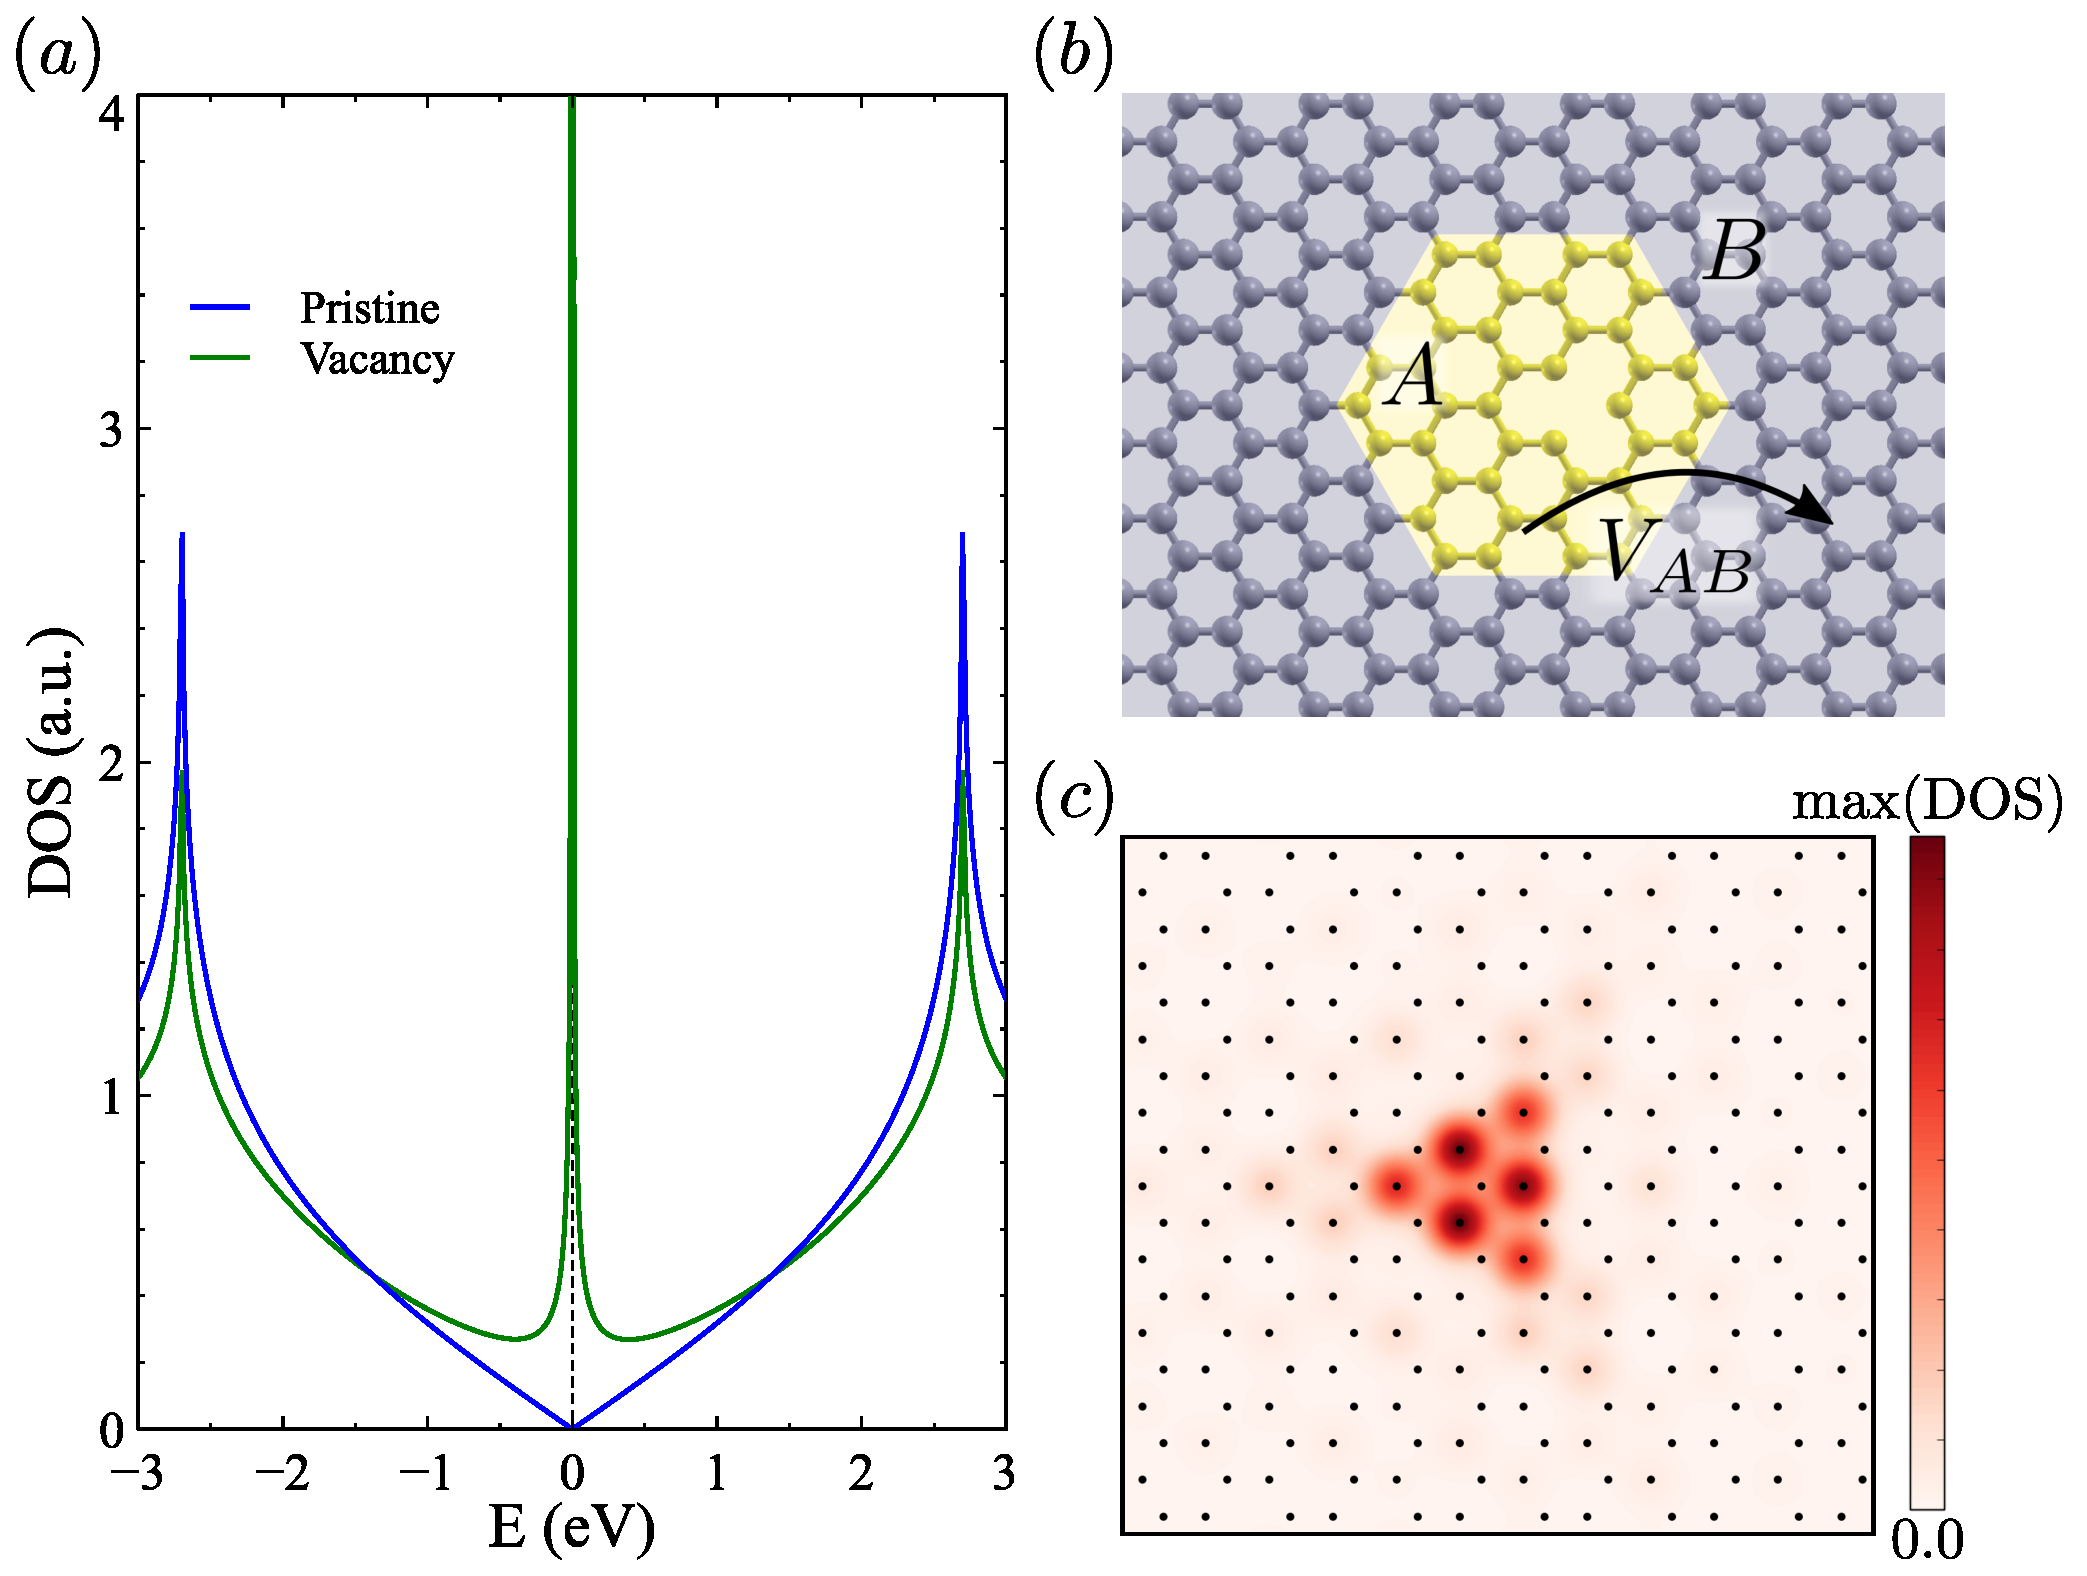
\includegraphics{defects/fig/DOSlDOS.pdf}
\caption{$(a)$ Total density of states of a single vacancy in an infinite graphene sheet. A divergence in the density of states appears at $E=0$ when the vacancy is introduced. $(b)$ Scheme of the division of the system into a defected unit cell and a pristine environment. $(c)$ Local Density of States for the zero energy state related to a vacancy in graphene. Side by side we can compare the calculations for two unit cells with different geometry. The vacancy is depicted as a white circle. As expected the spatial distribution of this state is located in the 3-6 closest atoms to the vacancy.}
\label{regions}
\label{DOS}
\vspace{-5pt}
\end{figure}
%~~~~~~~~~~~~~~~~~~~~~~~~~~~~~~~~~~~~~~~~~~~~~~~~~~~~~~~~~~~%
%%
We start by dividing the system into two regions, a central unit cell $A$ containing the defect, and the rest of the system $B$, containing everything else, as depicted in Fig.~\ref{regions} (b).
The Hamiltonian of the whole (infinite) system can then be written in terms of the two separated contributions, one arising from each isolated region, $H_0$, and the other arising from the coupling between the two regions $W$:

\begin{equation}
  H = H_{0} + W = \left(\begin{array}{cc}
   H_{A} &  0  \\
    0     & H_{B}
  \end{array}\right)+
  \left(\begin{array}{cc}
    0 & V_{AB} \\
   V_{BA} & 0
  \end{array}\right)
\end{equation}

The Green's function corresponding to region $A$ can be written (exactly) as:

\begin{equation}
  G_{A}(E) %= \frac{1}{E-H_{A}-V_{AB}\frac{1}{E-H_{B}}V_{BA}}
  = \frac{1}{E +i\eta - H_{A}-\Sigma_{AB}(E)}
  \label{Gdyson}
\end{equation}
where the \emph{embedding self-energy} $\Sigma_{AB}$ can be calculated from the Green's function of region $B$ %, decoupled from region $A$,
$g_B(E)=(E+i\eta-H_B)^{-1}$, as $\Sigma_{AB}(E)=V_{AB}\;g_B(E)\;V_{BA}$.
For numerical reasons $\eta$ has to be finite but we checked that the results do not depend on its exact value. We found that $\eta=0.001$ offers a good combination of precision in energy while keeping the convergence time of the Dyson equation reasonable.
In general the Green's function $g_B(E)$ for region $B$
% , and thereby the corresponding embedding self-energy $\Sigma_{AB}$,
are not straightforward to calculate, as $g_B(E)$ describes the Green's function of an infinite system without translational symmetry, on account of the missing region $A$.
However, the calculation of $\Sigma_{AB}$ is made possible when we consider two facts. First, $\Sigma_{AB}$ does not depend on whatever is in region $A$, second, equation \eqref{Gdyson} holds true for a pristine system with translational invariance, that permits to compute $G_A(E)$, and evaluate $\Sigma_{AB}=E- H_A-(G_A(E))^{-1}$.


The evaluation of $G_A(E)$ is now done by dividing the infinite pristine crystal system into periodic supercells $A'$ of the same size and shape as the defect region $A$.
The Green's function of region $A'$ in the perfect crystal can thus be calculated by integrating the $\vec{k}$-dependent Green's function in the whole Brillouin zone
\begin{equation}
  G_{A'}(E) =
\frac{1}{(2\pi)^2}
\int_{\text{BZ}} (E+i\eta-H(\vec{k}))^{-1} d^2\vec{k}
  \label{Gbloch}
\end{equation}
with $\vec{k}$ {the Bloch wavevectors}
and $H(\vec{k})$ the Bloch Hamiltonian for the pristine host
crystal. The final expression for the self-energy $\Sigma_{AB}$ reads:
\begin{equation}
  \Sigma_{AB}(E) = E+i\eta - H_{A'} -
\frac{1}{(2\pi)^2}
\left ({\int_{\text{BZ}}
(E+i\eta-H(\vec{k})})^{-1}d^2\vec{k} \right )^{-1}
\label{selfenergy}
\end{equation}
where $H_{A'}$ describes a region with the same dimensions than the original defective region $A$, but without the defect(s). This is a general procedure and can be applied for multi-band Hamiltonians. As long as the dimensions of the pristine and the defected Hamiltonian are the same, it can deal with more than one defect without computational overhead. Notice that this method does not require the analytic evaluation of the host crystal Green's function necessary in a recently proposed method\cite{settnes2015}, and can be applied to a very large class of systems, including superconductors.\cite{lado2016}

The combination of equations \eqref{Gdyson} and \eqref{selfenergy} allows the computation of the Green's function of the defective area, $G_A$, embedded in an otherwise pristine crystal as shown in Fig.~\ref{regions}. The density of states (DOS) of an atom $i$ in region $A$ can then be calculated from the imaginary part of the Green's function as
\begin{equation}
  % \rho_{i}(E) = -\frac{1}{\pi}\Im{\langle i| G_{A}(E)|i\rangle}
  \rho_{i}(E) = -\frac{1}{\pi}\Im{G_{i,i}(E)}
  \label{eq:DOS}
\end{equation}
where $G_{i,i}$ is the diagonal matrix element $(i,i)$ of the Green's function. Summing over the contributions from all atoms $i$ in region $A$, the total DOS of region $A$ is obtained.

In Fig.~\ref{DOS} we show the results of the method for the case of a single vacancy in the honeycomb lattice. Fig.~\ref{DOS} (a) shows the density of states both for pristine graphene, that shows the characteristic $\rho \propto |E|$ around the Dirac point,\cite{Katsnelson2012} and for the defective case, that presents a diverging zero energy resonance. The embedding method permits also the calculation of the local density of states as shown in Fig.~\ref{DOS} (c), where we show the map of the density of states evaluated at $E=0$, finding that the main contribution for this state comes from the 3-6 nearest neighbors to the vacancy that belong to the sublattice opposite to the one of the missing site.\cite{Pereira2006,kumazaki2007,Wehling2007,Pereira2008,Palacios2008}
Of course, for the case of a non-interacting single vacancy, this problem can be dealt with using the standard T matrix theory.\cite{libro-Economou,Gonzalez2012,Wehling2007}. The embedding method shows its added value when it comes to treat several vacancies or when interactions are included, as we discuss now.


\subsection{Mean field Hubbard model }
The Hubbard term acting on every site $i$ reads:
%%
\begin{equation}
  H_{U} = U \sum_i n_{i,\uparrow}\,n_{i,\downarrow}
\end{equation}
%%
where $n_{i\sigma}$ is the standard number operator for site $i$ with spin $\sigma$.
Exact solutions of this model are, in general, not possible so that we use a mean field approximation:
%%
\begin{equation}
  H_{U} \approx \sum_i
  U \left[\langle n_{i,\uparrow} \rangle n_{i,\downarrow} +
    \langle n_{i,\downarrow} \rangle n_{i,\uparrow}  -
    \langle n_{i,\downarrow} \rangle \langle n_{i,\uparrow} \rangle
  \right]
\end{equation}
where $\langle n_{i,\sigma} \rangle$ stand for the expectation values of the number operators computed with the eigenstates of the mean field Hamiltonian.
Of course, this is a non-linear problem that is solved self-consistently.  Here, this is done in combination with the two dimensional embedding technique, which is formally similar to the one dimensional case.\cite{munoz2009}
In this approach, the occupations in the external region $B$ are frozen to $\langle n_{i,\uparrow}\rangle= \langle n_{i,\downarrow}\rangle=\frac{1}{2}$.  In contrast, the expected values of the defective cell are calculated by self-consistent iteration.


In a first step, we assume a random guess spin polarization and then compute the expected values of the spin operators $\langle n_{i,\sigma} \rangle$ by integrating the DOS up to the Fermi energy
\begin{equation}
 \langle n_{i,\sigma}\rangle= \int_{-\infty}^{E_F} \rho_{\sigma}(E) dE
 \label{occ}
\end{equation}
which defines a new Hamiltonian for region $A$,$H_A \rightarrow \bar H_A + H^{MF}_U$%(\{m_i\})$
, including the mean field Hubbard term.\cite{Fernandez2007,Palacios2008} Notice that the numerical integration of eq. \eqref{occ} is much more efficiently done in the complex plane using Cauchy's integral theorem. Also it is important to notice that even when the Hamiltonian for the region $A$ will change over the self-consistent iterations the self-energies will not since they do not depend on what is inside of said region.
This procedure is iterated until a self-consistent solution is found.

The magnetic moment is calculated as the difference of the expected values of each spin densities.
\begin{equation}
\langle m(i)\rangle \equiv g\mu_B\frac{\langle n_{i,\uparrow}\rangle-\langle n_{i,\downarrow}\rangle}{2}
% \langle s_z(i)\rangle \equiv\frac{\langle n_{i,\uparrow}\rangle-\langle n_{i,\downarrow}\rangle}{2}
\label{sz}
\end{equation}

There is a trade off between computational cost, due mainly to the size of the region $A$, and the accuracy of the description of the semi-localized nature of the induced magnetism. The role of the chosen size for region $A$ is discussed bellow.


\subsection{The kernel polynomial method}
The Kernel polynomial method\cite{Weisse2006} is a spectral method that allows to calculate spectral properties of very large matrices without explicit diagonalization or inversion of the matrix.
This makes the method especially suitable for very large systems described by sparse Hamiltonians, as is the case for the first neighbor hopping model for the honeycomb lattice, considered here.
In our case, we set up the Hamiltonian for an extremely large graphene island, with a single vacancy in the center.

{The Chebyshev polynomials form a complete basis in the function space, so that they can be used as a basis to expand any well behaved function} $f(x)$ for $x\in (-1, 1)$
The method consists in expanding the density of states in $N$ Chebyshev polynomials $T_n(x)$,  that are calculated using $T_0(x)=1$, $T_1(x)=x$ and the recursive relation
\begin{equation}
T_{n+1} (x) = 2 x T_n(x) - T_{n-1} (x)
\end{equation}
valid for $x\in (-1,1)$.

The first step in the method is to  scale the Hamiltonian $H \rightarrow \bar H=\sum_k\bar E_k \ket{k}\bra{k}$
so that all the eigenstates $\bar E_k$ fall in the interval $\bar E_k \in (-1,1)$.  The density of states as a function of the scaled energy, at site $i$,  is expressed as
\begin{equation}
\rho_i(\bar E) = \frac{1}{\pi \sqrt{1-\bar E^2}}
\left (\bar \mu_0 + 2 \sum^{N-1}_{n=1} \bar \mu_n T_n (\bar E)
\right )
\label{KPM}
\end{equation}
The coefficients $\bar \mu_n$ are
the modified coefficients of the expansion,
\begin{equation}
\bar \mu_n = g^N_n \mu_n
\end{equation}
that are obtained using the Jackson kernel\cite{jackson1912approximation}
\begin{equation}
g_n^N =
\frac{(N-n-1)\cos \frac{\pi n}{N+1} + \sin \frac{\pi n}{N+1}
\cot \frac{\pi }{N+1}}{N+1}
\end{equation}
that improves the convergence of the expansion. The original
Chebyshev coefficients are calculated as a conventional
functional expansion
\begin{equation}
\mu_n = \int_{-1}^{1} T_n(\bar E) \sum_k \delta (\bar E-\bar E_k) |\langle k | i \rangle |^2
= \langle i | T_n(\bar H) | i \rangle
\label{mun}
\end{equation}
with $| i \rangle$ the wave function localized in site $i$. Importantly, the
second equality in eq. (\ref{mun}) relates $\mu_n$ to an expression where the
eigenstates $|k\rangle$ of $H$ are absent. Thus, diagonalization of $H$ is not
necessary and  the computation of the the $\mu_n$ coefficients only requires
calculating an overlap matrix element involving $T_n(H)$.
The Chebyshev recursion relation allow to write down the $\mu_n$ coefficients in term of the overlaps with the vectors $\ket{\alpha_n}$
\begin{equation}
\mu_n =
\braket{\alpha_0}{\alpha_n}%\langle \alpha_0 | \alpha_n \rangle
\end{equation}
generated by the recursion relation
\begin{equation}
\begin{aligned}
\ket{\alpha_0} = \ket{i}  \\  %|\alpha_0 \rangle = | v_i \rangle \\
\ket{\alpha_1} = \bar{H} \ket{\alpha_0} \\
\ket{\alpha_{n+1}} = 2\bar{H} \ket{\alpha_n}- \ket{\alpha_{n-1}}
\end{aligned}
\end{equation}
In our case, we will choose a state, $\ket{i}$, localized in the first neighbor
of the carbon with the hydrogen ad-atom.
To calculate the previous coefficients we only need matrix vector products,
so that the scaling is linear with the size $L$ of the system, in contrast with
the $L^3$ scaling for exact diagonalization.
Our calculations are performed in a graphene island with 800000 atoms,
taking a expansion with $N=10000$ polynomials.




\section{Non interacting zero temperature magnetization}
\label{sec:Phys}
In this section we study the spin polarization in the neighborhood of a $sp^3$ defect, driven by an external in-plane magnetic field coupled to the electronic spin, at zero temperature and in the non-interacting limit $U=0$.
In a gapped graphene system, this problem is straightforward. At $T=0$,  the
spin density would be dominated by the contribution of the only singly occupied
state, the $E=0$ mid-gap state, whose wave function we denoted by $\psi_0(i)\equiv \braket{i}{\psi_0}$.
The zero temperature magnetization in an atom $i$ would be given by:
\begin{equation}
m_i(B) = g\mu_B \left(\Theta(B)-\frac{1}{2}\right) |\psi_0(i)|^2
% |\braket{\psi_0}{i}|^2
\end{equation}
where $B$ is the magnitude of the magnetic field, $\Theta(B)$ is the step function, $g\simeq2$ is the gyromagnetic ratio and $\mu_B$ is the Bohr magneton. The local magnetization $m_i$ is stepwise constant, and discontinuous at $B=0$, $m_i(0^+)-m_i(0^-)= g\mu_B |\psi_0(i)|^2$.
It is apparent that the total moment $M=\sum_i m_i$ integrates to $M=\pm \frac{g\mu_B}{2}$ on account of the normalization of the wave function of the mid-gap state. This result holds true as long as the Zeeman energy $\mu_B B$  is smaller than the gap of the structure.

%~~~~~~~~~~~~~~~~~~~~~~~~~~ FIGURE 2 ~~~~~~~~~~~~~~~~~~~~~~~~~%
\begin{figure}[t!]
  \centering
  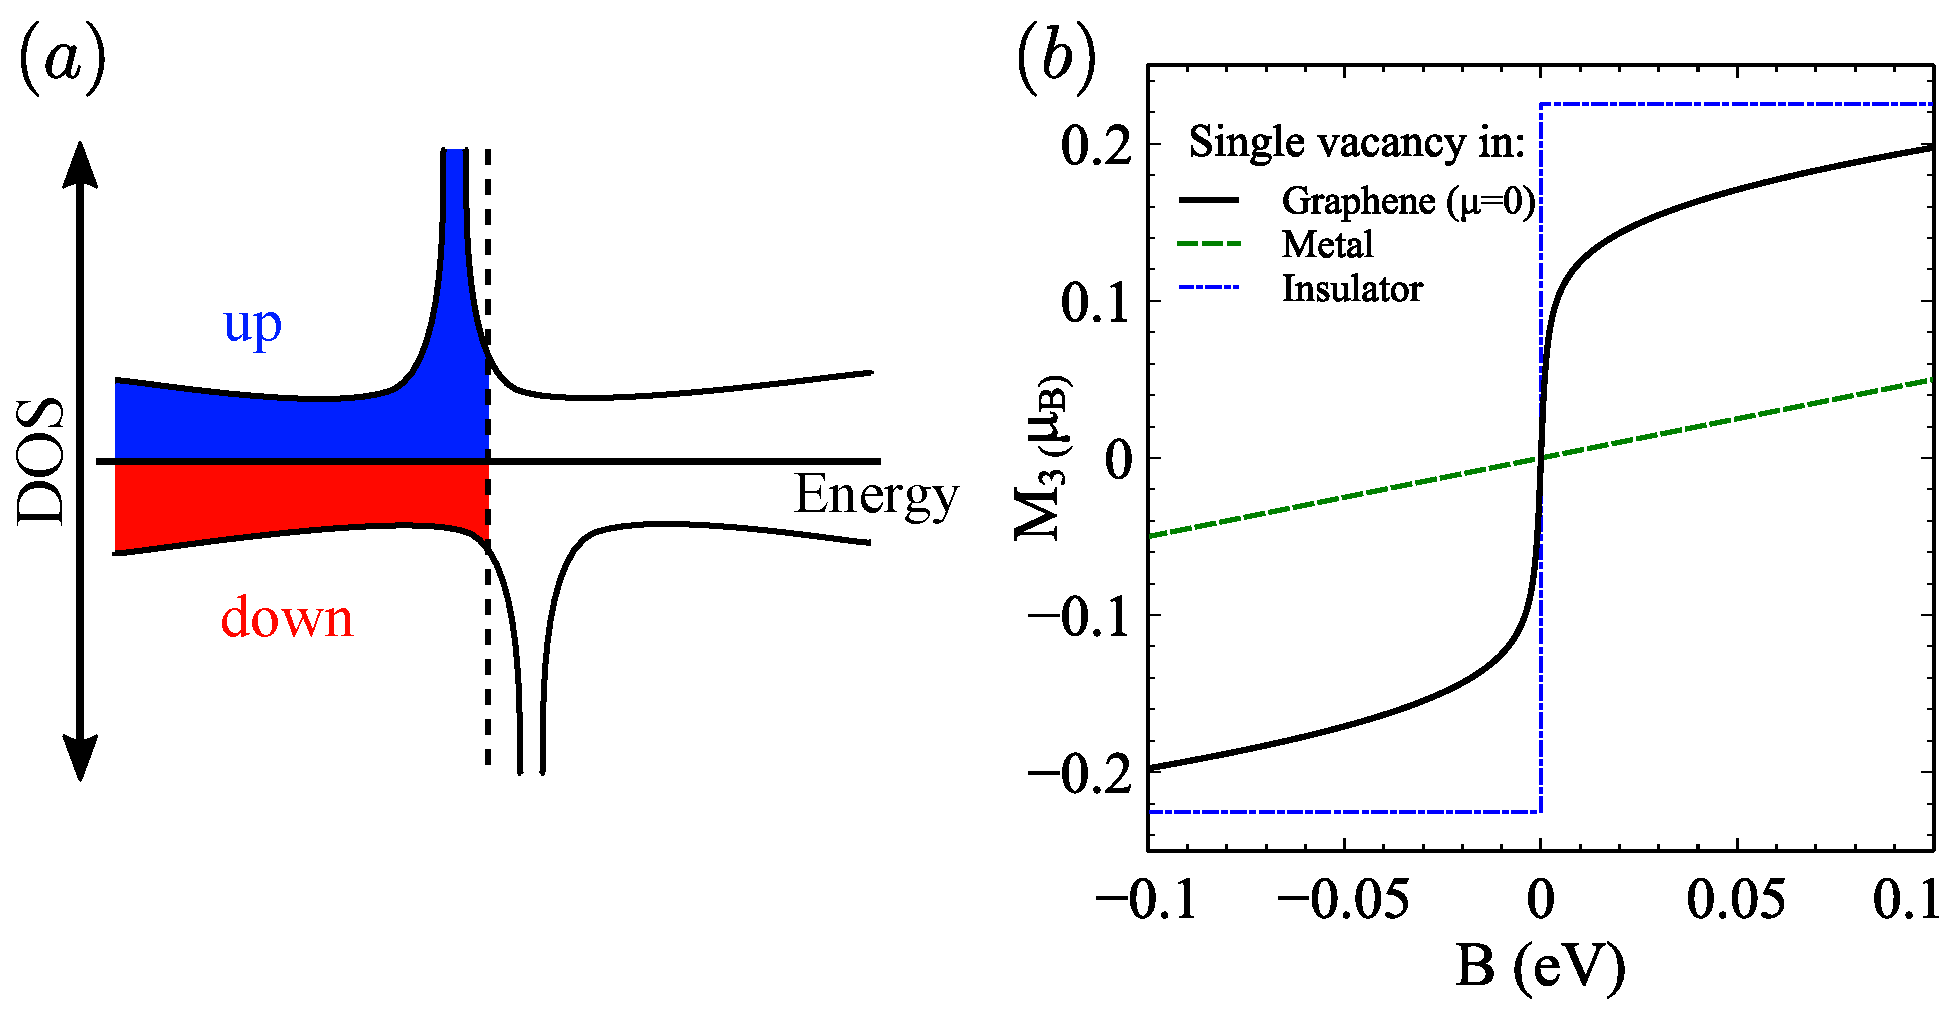
\includegraphics{defects/fig/comparison.pdf}
  \caption{$(a)$ Sketch for the Zeeman split  DOS associated to  graphene with an individual $sp^3$ functionalization. Panel $(b)$ shows the magnetization of the first 3 neighbors of the defect as a function of the applied magnetic field for a hydrogen atom in a graphene quantum dot (blue) and a single hydrogen atom in pristine graphene (black), the green line is the result for a conventional metal, modeled by graphene with the chemical potential well above the Dirac point.}
  \label{mb}
\end{figure}
%~~~~~~~~~~~~~~~~~~~~~~~~~~~~~~~~~~~~~~~~~~~~~~~~~~~~~~~~~~~%
%%
We now study what happens in the case of infinite pristine graphene, for which there is no gap, and we cannot define a normalized zero energy state. For that matter, we compute the density of states of the system using the Green's function embedding approach % and the kernel polynomial method.
This methods is trivially adapted to include the Zeeman splitting that introduces a rigid spin dependent energy shift $\pm\mu_B B$. This symmetric shift allows the expression of all the spectral functions for each of the spin channels in terms of the spinless Green's function, $G^\sigma(E)=G(E-\sigma \mu_BB)$, with $\sigma= \pm 1$.

% Thus, for $T=0$, we use the equations \eqref{occ} that permits to relate the integrated density of states to the local magnetic moment
% \begin{equation}
% \langle m_i\rangle = g\mu_B \frac{\langle n_{i,\uparrow}\rangle-\langle n_{i,\downarrow}\rangle}{2}
% \end{equation}

The results for the magnetization of the three first neighbors of a $sp^3$ defect in an otherwise pristine graphene are shown in Fig.~\ref{mb} for a single $sp^3$ defect in two scenarios. A gapped finite size graphene hexagonal island with armchair edges, resulting in the expected step-wise response, a single defect in otherwise pristine gapless graphene.
In both cases we plot  the magnetization of the three atoms closest to the vacancy,
% $\overline{m}=\sum^3_{i=1}m_i$
$M_3=\sum^3_{i=1}m_i$, that gives the dominant contribution to the
defect-induced local moment. {The result for the paramagnetic response of a
metal is included in Fig.~\ref{mb} for comparison with a standard case}.

The most prominent feature of the obtained results is the fact that the
% $\overline{m}(B)$
$M_3(B)$ curve is not stepwise constant for the defect in infinite graphene, in marked contrast with the case of the defect in a gapped island.
This difference shows the qualitatively different behavior of the zero mode in gapless infinite graphene, compared to the standard case of an in-gap truly localized state. The \emph{continuous variation} of the magnetic moment can be related to the fact that the zero mode has an intrinsic line-width that reflects the lack of a gap to host a true localized state.

% The results for infinite graphene depend on the small imaginary part $\eta$ that has to be added to the energy argument $E$ of the Green's functions, for a matter of numerical convenience. Several different values of $\eta\in [0.1,0.0001]$ where tested finding the results consistent in all of the calculations.
% {The value chosen was $\eta=0.001$ which offers a good combination of precision
% in energy while keeping the convergence time of the Dyson equation reasonable.}



\section{Finite temperature susceptibility}
\label{sec:Temp}
We now discuss the effect of temperature on the non-interacting $m(B)$ curve. The only effect of temperature is to smear out the occupation of the one-particle levels, so that the expected value of the local magnetization has to include now excited states.

To calculate the magnetization in a site $i$  as a function of the magnetic field and the temperature we just need to compute the difference in the occupation of the spin-up and spin-down density of states weighted with the Fermi-Dirac distribution function. Thus, the local magnetic moment is given by $m_i = g\mu_B \langle s_z(i) \rangle$ with
\begin{equation}
       \langle s_z(i) \rangle = \frac{1}{2}
      \int^{\infty}_{-\infty}\left[
      \rho_{i\uparrow}(E)-\rho_{i \downarrow}(E)
      \right] f(E,T) dE
\label{mag_b_t}
\end{equation}
where $f(E,T)$ is the Fermi Dirac distribution and $\rho_{i\sigma}(E)$ is the
spin resolved density of states. The resulting magnetization of the three
closest atoms, $M_3$ is shown in Fig.~\ref{mag_temp} (a), computed with two
different approaches, the embedding method for a single $sp^3$ defect in
infinite graphene and the kernel polynomial method for a single defect on a
finite size island with a very large number of atoms.
It is apparent that both methods give identical results in the chosen range of temperatures.

In order to highlight the anomalous behavior of the magnetic  moment associated to an individual $sp^3$ defect, we focus on the spin susceptibility, defined as
\begin{equation}
  \chi(T) = \left.\frac{\partial m (T)}{\partial B}\right|_{B=0}
\label{susceptibility}
\end{equation}
For $T=0$ the results of the previous section show that this quantity diverges, both for the gapped and gapless cases. Here we study the dependence of $\chi(T)$ as a function of temperature $T$. For a conventional local moment,  the zero field susceptibility follows the Curie law $\chi(T) \propto T^{-1}$. This result holds true, based on very general considerations, for any spin governed by the Hamiltonian $g\mu_B  \vec{S}\cdot\vec{B}$ as well as any classical magnetic moment $\vec{M}$ governed by the interaction energy $-\vec{M}\cdot\vec{B}$. In particular, the Curie susceptibility of a single electron in an in-gap level will follow a Curie law.

%~~~~~~~~~~~~~~~~~~~~~~~~~~ FIGURE ~~~~~~~~~~~~~~~~~~~~~~~~~%
\begin{figure}[t!]
  \centering
  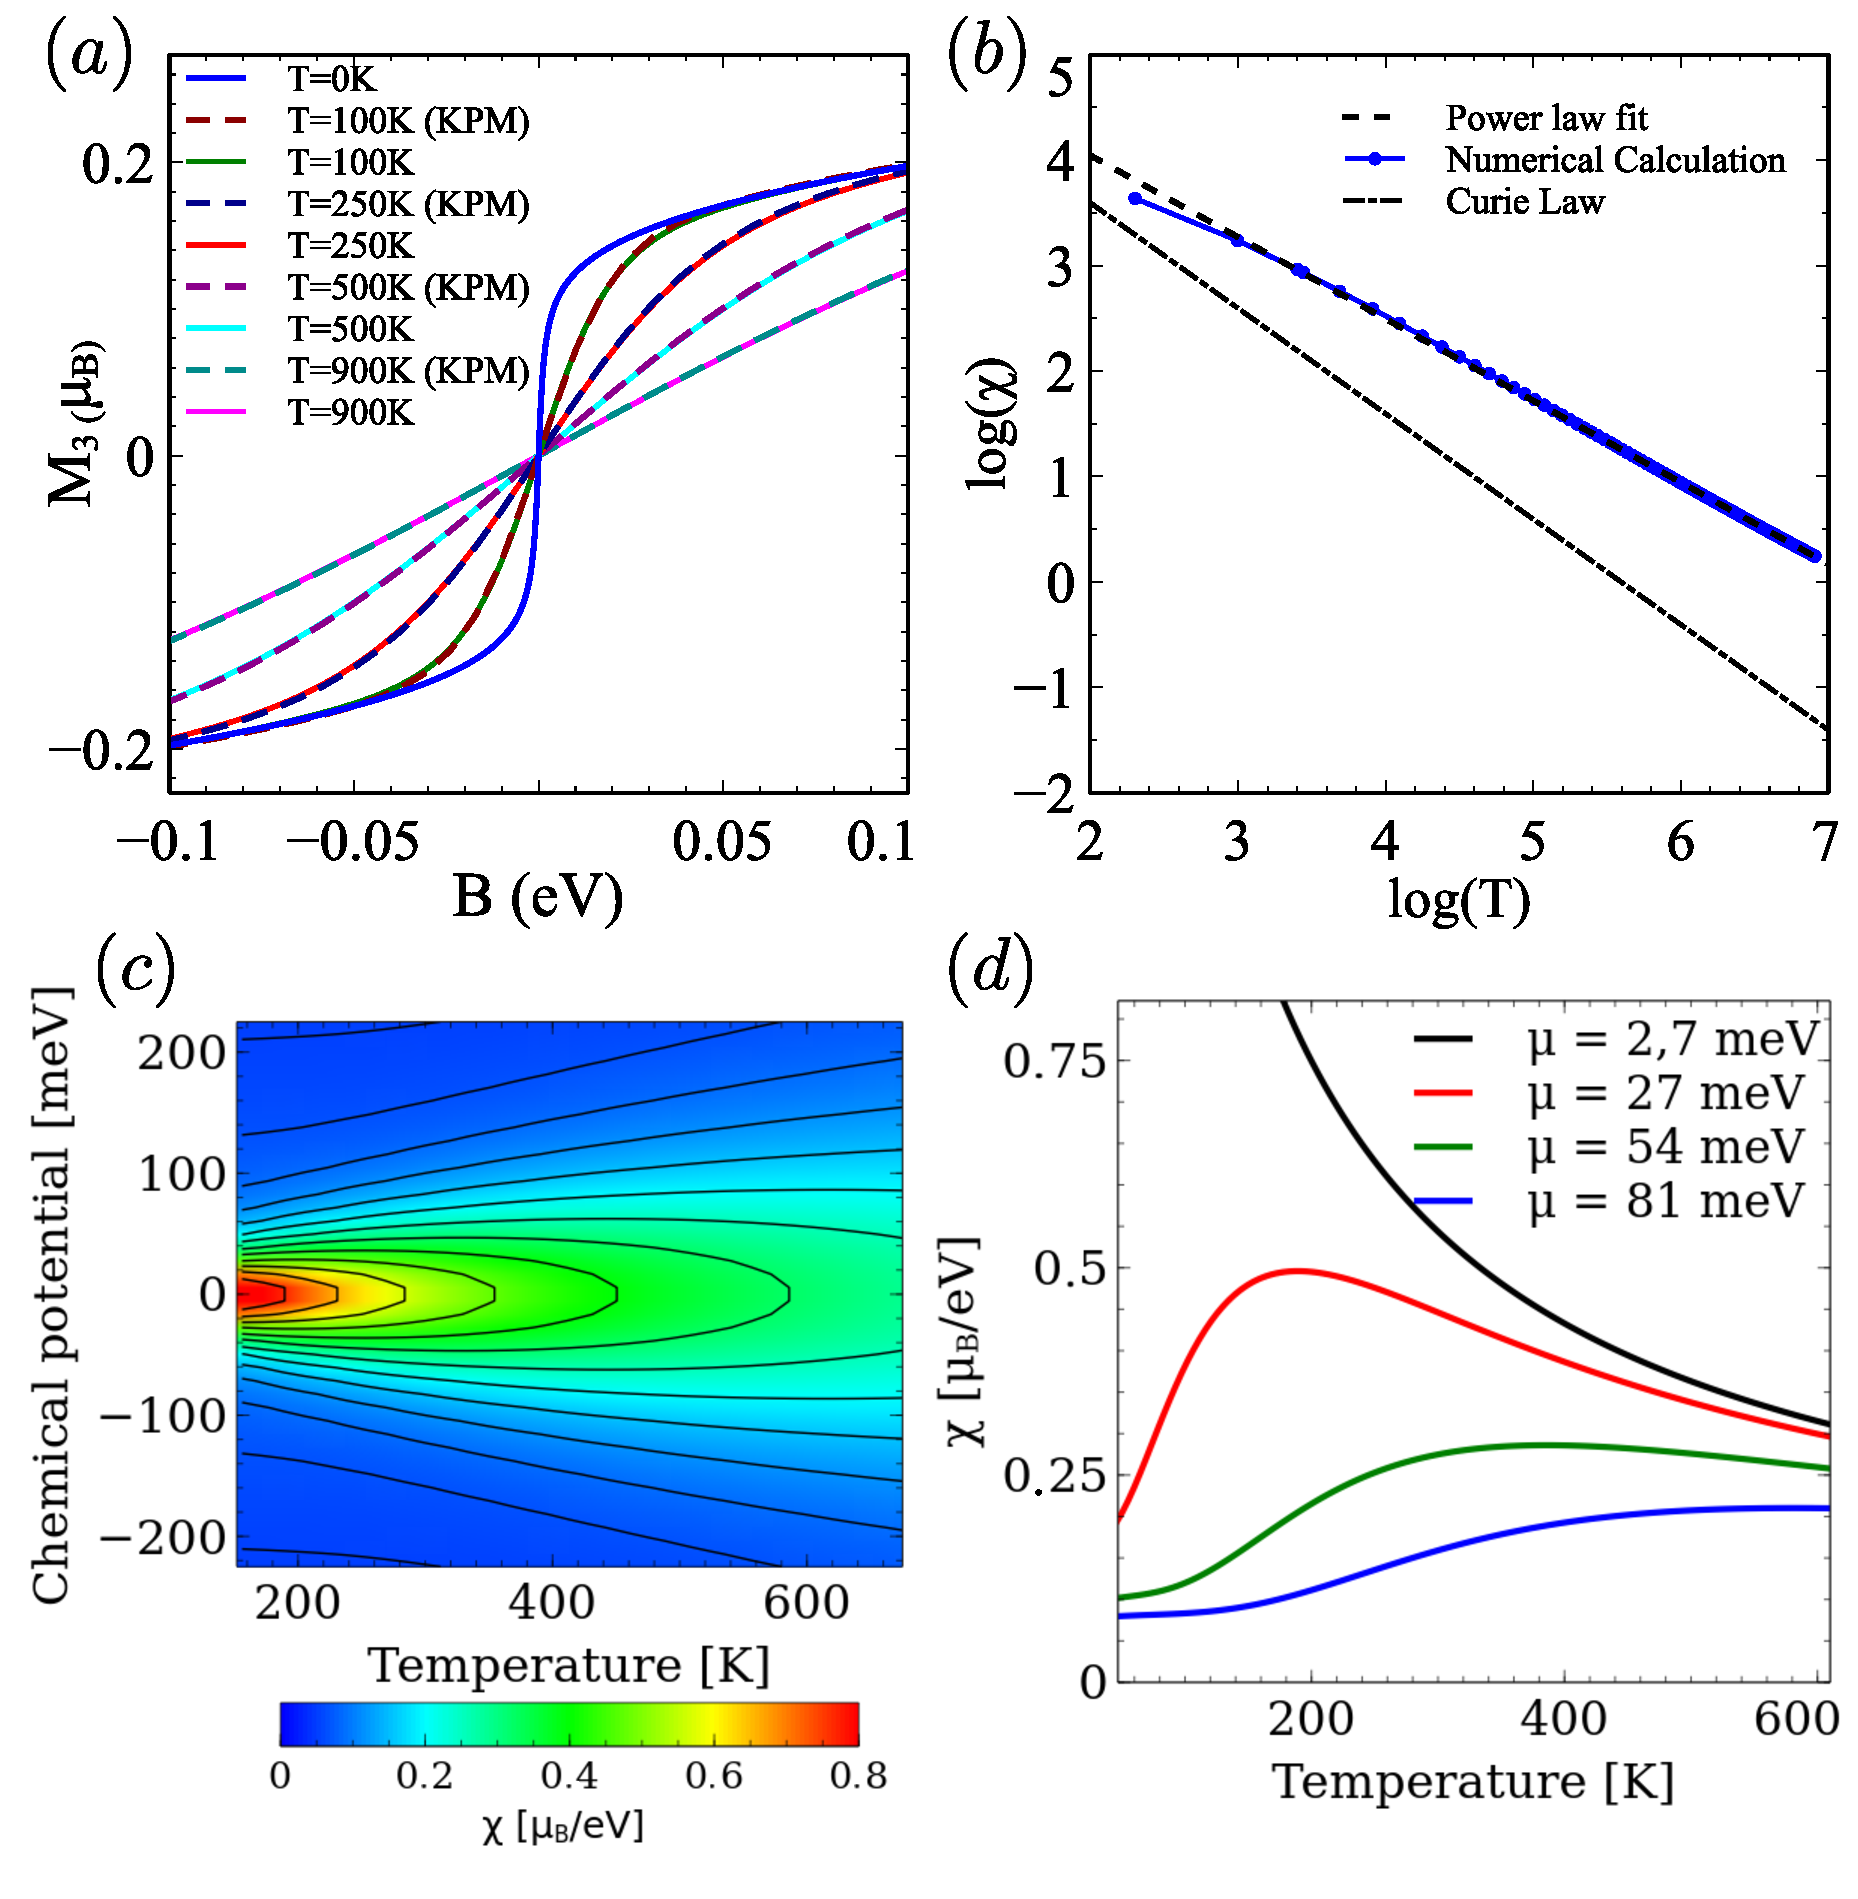
\includegraphics{defects/fig/temp_sus.pdf}
  \caption{$(a)$ Magnetization of the first 3 neighbors of the vacancy as a
    function of the applied magnetic field for different temperatures, dashed lines are calculated using the KPM and continuous lines are calculated using the embedding method. $(b)$ Temperature dependence of the susceptibility in comparison with Curie's Law. $(c$-$d)$ Dependence of the susceptibility with the doping and the temperature, showing that for some values of $\mu$ there is a non-monotonous behavior of the susceptibility with temperature.}
  \label{mag_temp}
\end{figure}
%~~~~~~~~~~~~~~~~~~~~~~~~~~~~~~~~~~~~~~~~~~~~~~~~~~~~~~~~~~~%


Numerical derivation of the results of  Fig.~\ref{mag_temp} (a) allows the calculation of $\chi(T)$, shown in Fig.~\ref{mag_temp} (b) in a Log-Log representation.
It is apparent that the spin susceptibility for the $sp^3$ defect on graphene
\emph{does not follow} the Curie law.
In particular, we obtain a high temperature power law dependence $\chi \propto T^{-\alpha}$, with $\alpha\sim0.77$, in comparison with the conventional $\alpha=1$.
This exponent reflects, again, the anomalous nature of the $sp^3$ local moment in infinite graphene, in marked contrast with the behavior of the same chemical functionalization in a gapped graphene structure.
Interestingly, $\chi(T)$ has been measured\cite{Nair2012} for defective graphene obtaining a Curie law dependence, probably because the samples used are in fact nanoflakes with small confinement gaps that permit the existence of in-gap states with quantized spins.

Further insight into the magnetic properties of this system is obtained by considering the dependence of the magnetic susceptibility as a function of the graphene chemical potential, that could be modified by gating doping,\cite{nair2013dual} as shown in Fig.~\ref{mag_temp} (c,d).
The maximal local susceptibility is obtained at half-filling and small temperatures where it monotonically decreases both with temperature and doping.
In comparison, in the case of slightly doped samples, the magnetic
susceptibility can either increase or decrease as a function of the
temperature, showing a maximum at a doping-dependent temperature. The previous
behavior can be understood as a crossover from the impurity in an insulator to
the metallic regime.
Importantly, the local maximum implies that graphene doping introduces an energy
scale that determines the temperature for the impurity-metal crossover. In the
case of heavily doped samples ($\mu = 81$ meV),
the susceptibility grows monotonically with temperature,
signaling the conventional metallic regime.



\section{Effect of interactions}
\label{sec:MF}
We now study the effect of electron-electron interactions in the formation of local magnetic moments associated to the $sp^3$ functionalization. A single unpaired electron in an in-gap energy level has a spin $S=1/2$ (equivalent ot a magnetic moment $m=1\mu_B$). In the current study this is not the case, the $E=0$ resonance is embedded in a region with finite DOS (except in just one point, the Dirac energy) and the existence of an emergent magnetic moment follows the Stoner criterion $U\rho(E_F)=1$. For graphene with a single $sp^3$ defect the diverging nature of $\rho(E)$ at $E=0$, the presence of arbitrarily small interactions gives rise to a local moment.
However, because of the coupling of the mid-gap state to a continuum of states (the linear bands of graphene) it is not obvious a priori whether or not the local moment should have a quantized $S=1/2$ spin.
In the following we address this issue, using the mean field approximation for the Hubbard model and the embedding technique as discussed in previous sections. The Hubbard model, while is not certainly the complete description of such a system, offers a simple model to gain an insight on the possible magnetic solutions for the systems.


\subsection{Local magnetic moment}
In general, the results of the mean field calculation yield a non-zero magnetization above rather small values of $U$. However, the integrated local moment $M=\sum_{i\in A} m_i$ is far below the quantized value of $M=1\mu_B$. A characteristic snapshot of the magnetization density computed for a simulation cell with 162 atoms within the mean field Hubbard model is shown in Fig.~\ref{MF} (a). The dominant magnetic moments appear in the sublattice opposite to the one of the defect, but small contributions of opposite sign appear in the same sublattice.
%%
%~~~~~~~~~~~~~~~~~~~~~~~~~~ FIGURE ~~~~~~~~~~~~~~~~~~~~~~~~~%
\begin{figure}[t!]
  \centering
    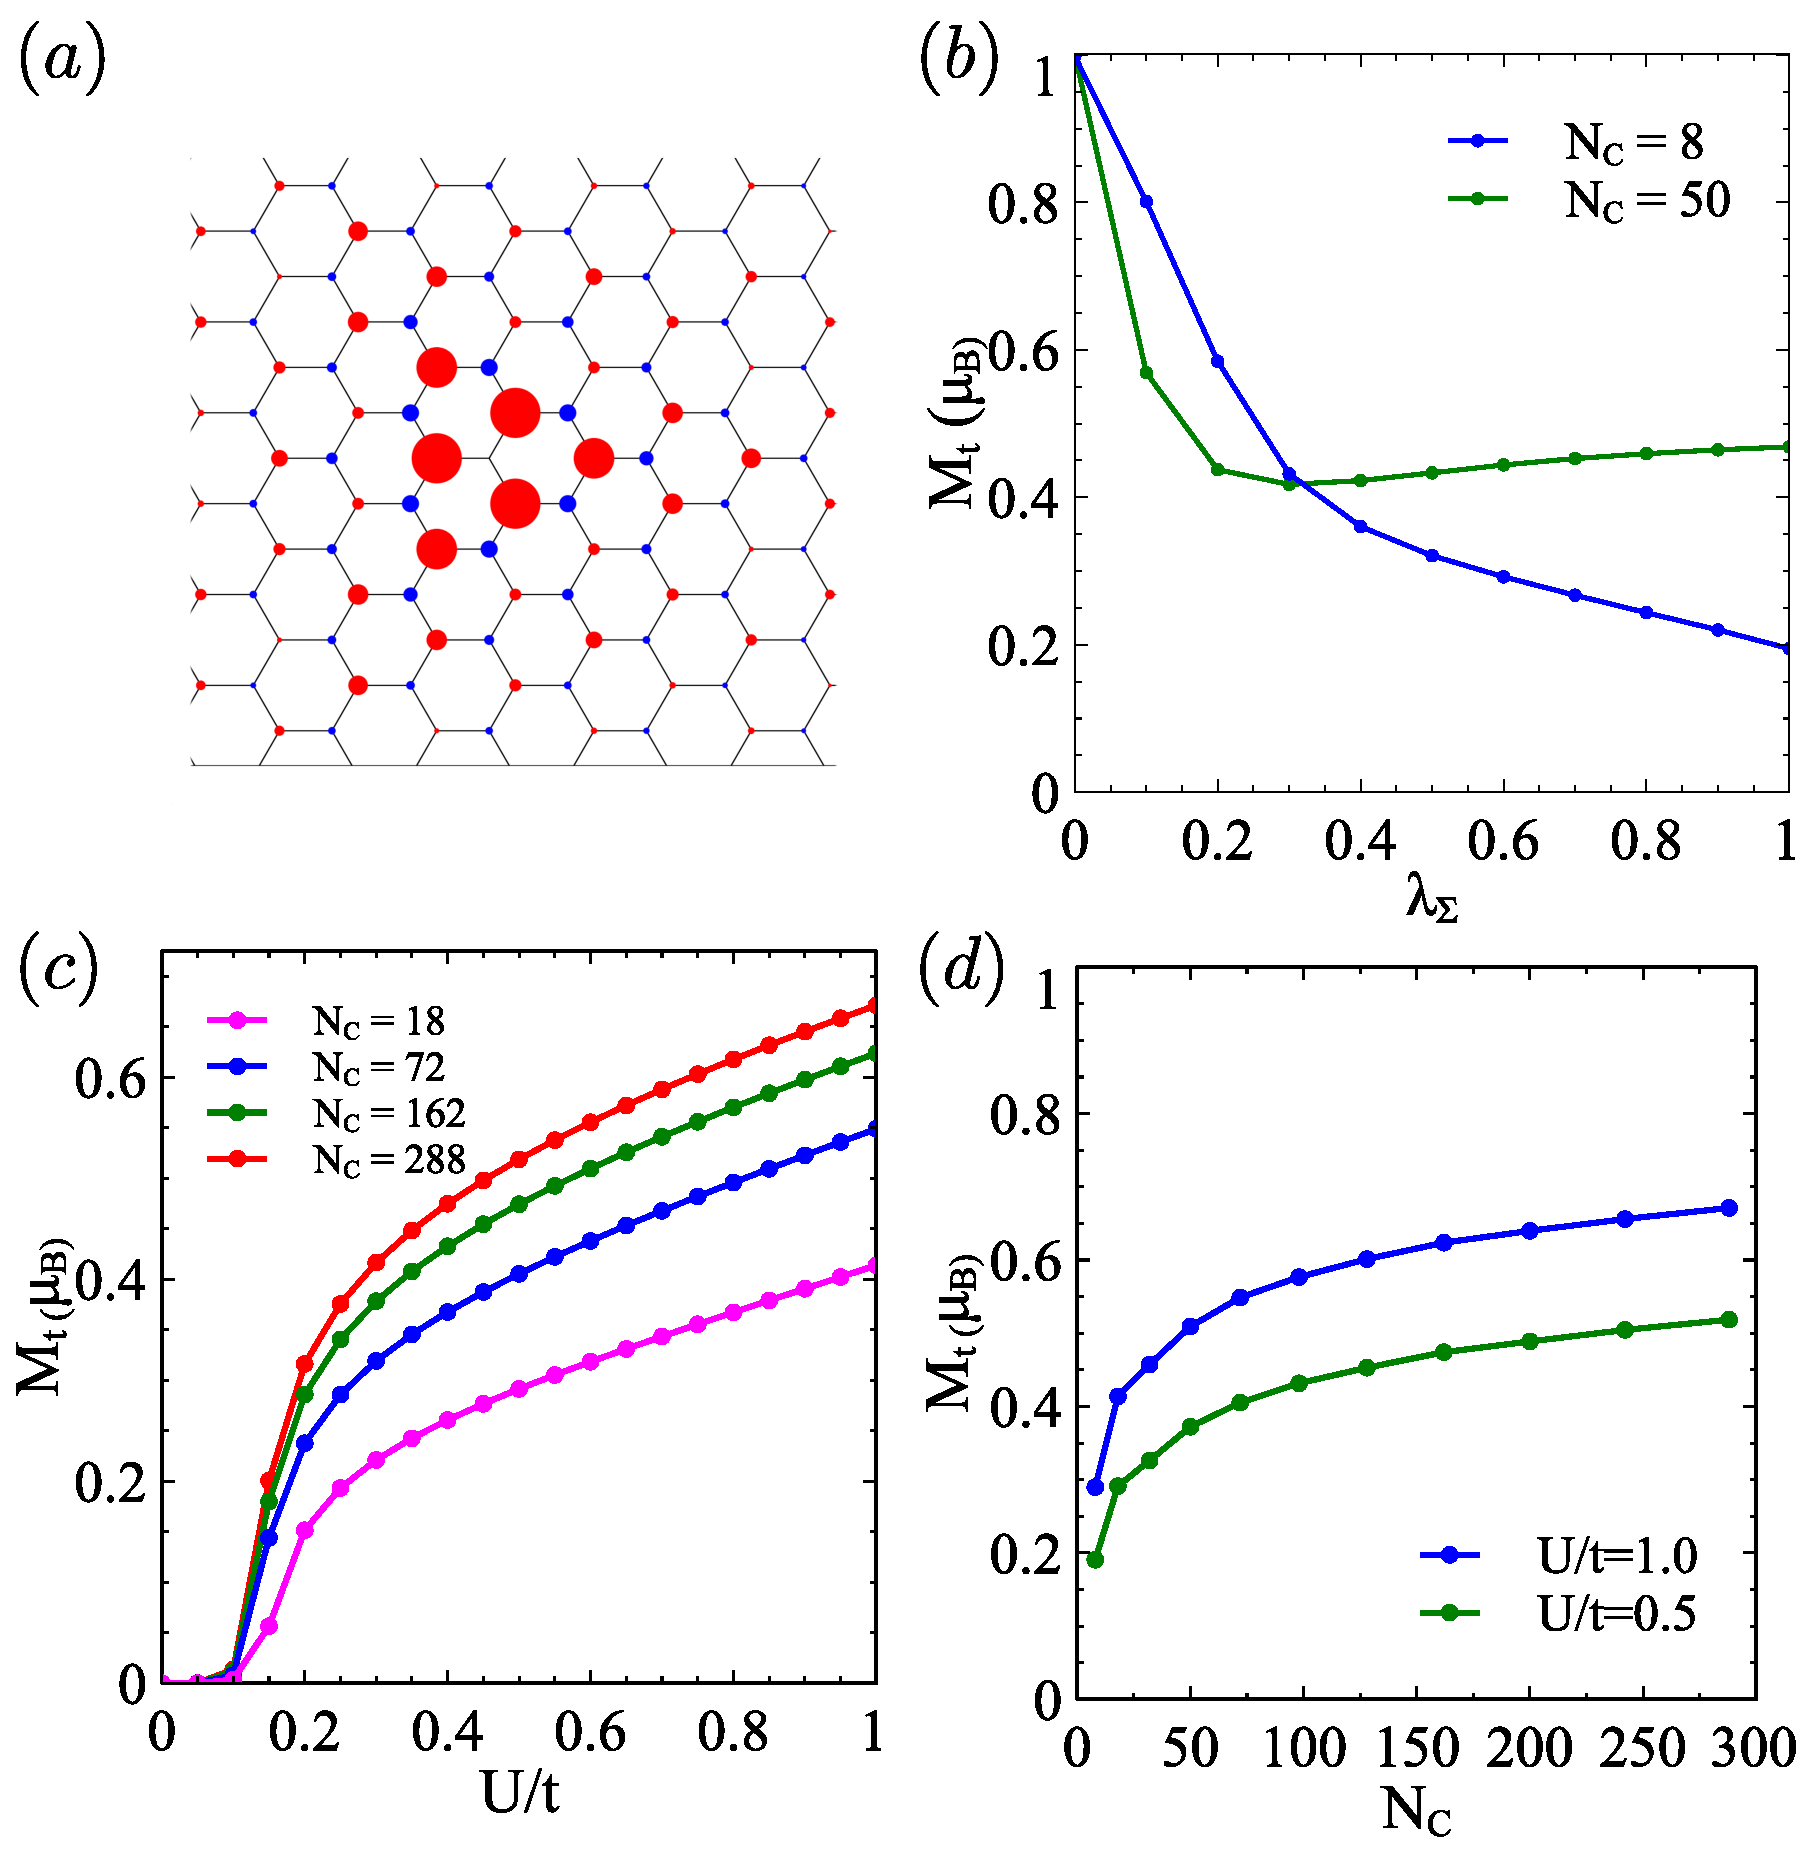
\includegraphics{defects/fig/figMF.pdf}
  \vspace{-15pt}
  \caption{$(a)$ Magnetization of an individual $sp^3$ functionalized system, calculated within the mean field  Hubbard  approximation. $(b)$ Total magnetization of the defected region as a function of its coupling to the rest of the otherwise pristine system. $(c)$ Total magnetization of the defected region as a function of the Hubbard $U$ for different sizes of the unit cells. $(d)$ Total magnetization as a function of the size of the unit cell for two $U$ values, notice that the magnetization is far from the expected $m=1\mu_B$ value.}
  \label{MF}
\end{figure}
%~~~~~~~~~~~~~~~~~~~~~~~~~~~~~~~~~~~~~~~~~~~~~~~~~~~~~~~~~~~%
%%
The influence of the coupling to infinite graphene is neatly shown in a calculation where we artificially tune the intensity of the interaction between the central simulation cell $A$, and the rest of graphene.
For that matter, we define the following modified full Green's function
%%
\begin{equation}
  \widetilde{G}_{A}^\lambda(E) =
  \frac{1}{E+i\eta-\widetilde{H}_{A}-\lambda_\Sigma\,\Sigma_{AB}(E)}
\end{equation}
%%
where $\lambda_\Sigma\in[0,1]$ is a control parameter that smoothly interpolates
between limit where the region $A$ is decoupled ($\lambda_\Sigma = 0$) from the rest of the universe, quantum dot regime, and the infinite-crystal regime
($\lambda_\Sigma = 1$).

As it is shown in Fig.~\ref{MF} (b), in the quantum dot regime $\lambda_\Sigma = 0$ the magnetic moment is quantized $M=1\mu_B$. However, as soon as the unit cell is coupled to the rest of the graphene, $\lambda_\Sigma \ne 0$, the magnetic moment rapidly becomes non-quantized, with an evolution that depends on the size and geometry of the region $A$.
%%
%~~~~~~~~~~~~~~~~~~~~~~~~~~ FIGURE ~~~~~~~~~~~~~~~~~~~~~~~~~%
\begin{figure}[h!]
\centering
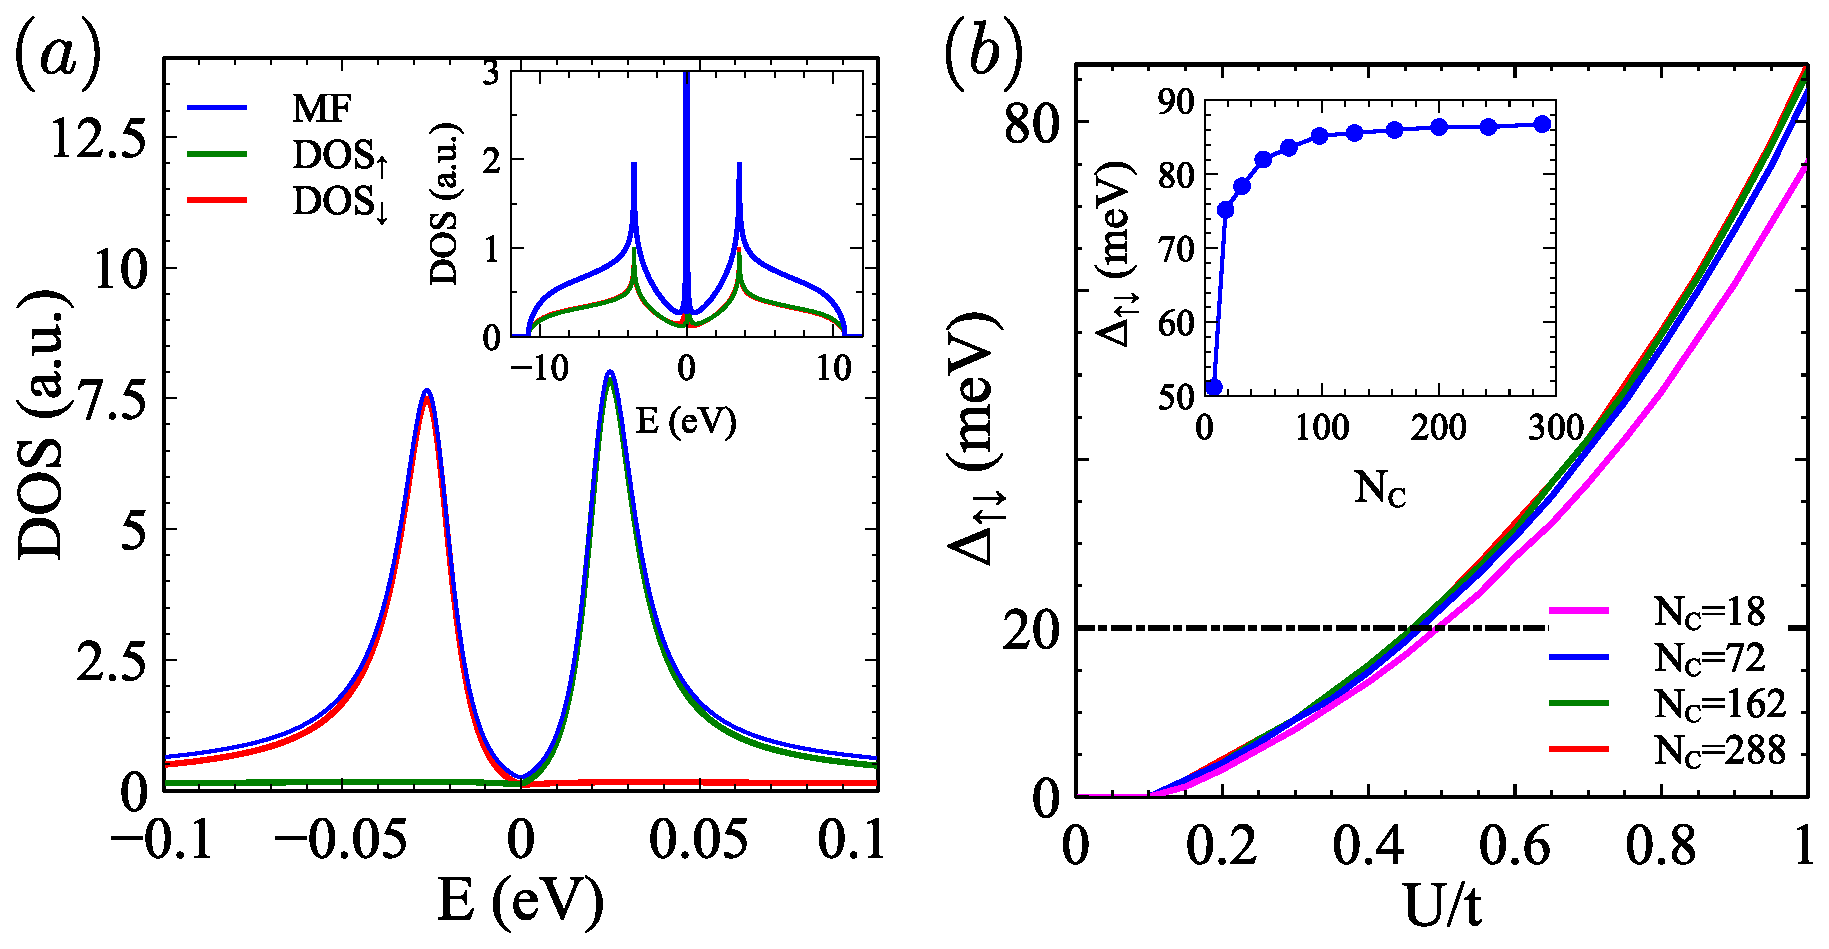
\includegraphics{defects/fig/MFfig2_dos.pdf}
\vspace{-15pt}
\caption{$(a)$ total and spin-resolved DOS for the Hubbard model. $(b)$ spin splitting, $\Delta$ as a function of the Hubbard interaction $U$ and, in the inset, as a function of the size of the unit cell.}
\label{MFdos}
\end{figure}
%~~~~~~~~~~~~~~~~~~~~~~~~~~~~~~~~~~~~~~~~~~~~~~~~~~~~~~~~~~~%
%%
As soon as $U$ is larger than a small critical $U\simeq 0.01 t$, magnetic solutions are obtained and we find that the non integer nature of the magnetic moment holds for a wide regime of electronic interactions $U$.
The net magnetic moment is an increasing function of $U$ as well as the size of the central region, $N_C$, Fig.~\ref{MF} (c,d). Even for the largest simulation cells, with up to 288 sites, the total magnetic moment remains clearly below $1\mu_B$. However, a representation of the total moment as a function of $N_C^{-1}$, not shown, makes it hard to predict whether or not the extrapolation to an infinite cell would recover the quantized value. Whereas it might be that the magnetic moment is quantized, our calculations emphasize the rather extended nature of this object.

\subsection{Spin splitting}
Our magnetic self-consistent solutions spontaneously break symmetry and result in spin-split density of states, shown in Fig.~\ref{MFdos}.
Importantly, the interacting DOS does not have any integrable singularity, as it happens for the $U=0$ case at $E=0$. Summing over spin projections, the total density of states still shows electron-hole symmetry.
However, the spin-resolved DOS is split, so for one spin projection the resonance is below the Fermi energy, while for the other one is above, which accounts for the net magnetization.
We define the spin splitting, $\Delta$, as the difference in energy between
these two resonances. We find that $\Delta$ has a super-linear dependence on
the Hubbard interaction $U$, as shown in Fig.~\ref{MFdos} (b). This reflects
the fact that the spin splitting is linear both in $U$ and in the magnetic
density $m$, which is also an increasing function of $U$. These results depend
weakly on the size of the defective region, $A$, in the embedding calculation
(inset of Fig.~\ref{MFdos} (b)).\\


We now address the connection between the DOS in Fig.~\ref{MFdos}(a), that shows two spin-split peaks around the Fermi energy,  and the STM $dI/dV$ spectra reported by Gonz\'alez {\em et al.}\cite{gonzalez2016atomic}.
Whereas the experimental $dI/dV$ curve also shows   two peaks,
the interpretation of the  experimental observations\cite{gonzalez2016atomic} requires some caution. The  spin-split peaks in the mean field calculation arise  from the   breaking of the spin symmetry.  This band splitting does indeed occur in    ferromagnetic systems  large enough to keep the magnetization frozen along a given direction that defines a spin quantization axis that permits the definition of the spin orientation of the spin-split bands. The quantum fluctuations of this mean field picture can be safely neglected for a large enough magnetic moment, but this is definitely not the case of a system that, at most, has $S=1/2$.


Therefore, the origin of the two peaks observed in the experiments
\cite{gonzalez2016atomic} is {\em not} the spin splitting of the graphene energy levels, in line with the discussion Gonzalez {\em et al.}\cite{gonzalez2016atomic}.  A more correct interpretation of the split peaks is the following. The STM $dI/dV$ is proportional to the spectral function of the surface, in this case,  graphene. The spectral function of a localized level has two peaks,  associated to the addition $E>E_f$ and removal $E<E_f$ of an electron in the system. Their energy difference is a measurement of the {\em addition energy} of the system, i.e., the Coulomb repulsion between the host localized electron and a second additional electron injected in the system. When the addition energy is larger than the temperature, as in the experiment, the system is in the so called Coulomb-Blokade regime. This entails the existence of an unpaired spin, very much like in the Anderson model\cite{anderson1961localized} and does not preclude the emergence of Kondo effect at very low temperatures. The proper treatment of the addition energies in this system would involve solving the single impurity problem of a resonance in a Dirac bath in a many body  framework\cite{haase2011magnetic,sofo2012magnetic,mitchell13}, which is out of the scope of the present work.

Finally, for a truly localized level with wave function $\phi_0$, described with the Hubbard model,  both the addition energy and the mean field spin-splitting are roughly given by  $U\sum_i |\psi_0(i)|^4$.  Therefore,  even if the spin-splitting  of the mean field theory is conceptually different from the addition energy observed experimentally, these two quantities roughly described by the same formula.



\subsection{Localization}
Our calculations show that magnetic moment associated to a hydrogen ad-atom is dellocalized in more than 250 carbon atoms.
In this sense, our calculations highlight the anomalous nature of the resonance due to a single $sp^3$ impurity in contrast to the phenomenology in gapped systems. This behavior arise from the special condition of the DOS, (null only in exactly one point) and the absence of an energy scale able to confine the $E=0$ resonance.


It is worth noting that in real graphene some effects not captured by the first neighbor Hubbard model that can play a relevant role. First, the existence of second neighbor carbon hopping breaks electron-hole symmetry and shifts  the vacancy state away from $E=0$. Second, single hydrogenation introduces an effective on-site energy in the carbon atom that is actually finite, although rather large, which also leads to a displacement of the resonance away from zero energy.
Third, non-local electronic interaction in graphene may have a sizable effect on the magnetic moment.
And finally, spin-orbit coupling would open a gap of around $0.03meV$.
\cite{PhysRevB.80.235431}
Whether any of the previous perturbations would be capable of moving the system to the conventional quantum dot regime would require a careful study with a first principles Hamiltonian, which is out of the scope of the present work.

\section{Conclusions}
\label{sec:Concl}
We have addressed the problem of the local moment formation induced by an individual $sp^3$ functionalization in graphene, with chemisorbed atomic hydrogen as the  main motivation.  We model this within the single orbital Hubbard model, so that the functionalization is modeled as a vacancy in the  honeycomb lattice.  We have shown that the magnetic moment in this system  departs from  the conventionally accepted $m=1\mu_B$ picture. This relates to the fact that the lack of a gap in graphene prevents the existence of a standard in-gap state that can host an unpaired electron. Our calculations show that the local moment induced by $sp^3$ functionalization in otherwise gapless and pristine graphene
 give rise to specific signatures in the magnetic response of the system, such as a non-Curie temperature dependence and a non-linear (and non-monotonic for
some doping values) magnetic susceptibility.
We have also shown by means of mean-field calculations that the resulting magnetic moment is non-quantized in the whole regime explored. Our results should pave the way for future work treating many-body spin fluctuations beyond mean field theory\cite{haase2011magnetic,sofo2012magnetic,mitchell13}




\section{Hyperfine tunability of a H adatom on graphene.}
While the model of an effective vacancy in the $p_z$ manifold is a very simple and useful model, it lacks some ingredients that can also provide interesting physical effects.

We are going to discuss briefly here the implementation of this system in a \ac{sk} framework as described in previous chapters.

We are going to neglect the $sp^3$ deformation of the lattice and consider simply that the $H$ atom has some hoppings to the $C$ orbitals. Due to the symmetry of the problem, both the $s$ and $p_z$ orbitals will have a finite hopping with the $s$ orbital while de $p_{xy}$ will not. In the \ac{sk} approximation, the effective hoppings will be governed by the parameters $V_{ss\sigma}$ and $V_{sp\sigma}$.

The most naive approach would be to use the \ac{sk} parameters detailed in previous chapters \ref{G_SK_params}. For the sake of the argument we will proceed that way.

%This hybridization results in the formation of bounding-antibounding states which shifts the $p_z$ orbital far away in energies, which is equivalent to the effective removal from one of the sites in the $p_z$ manifold.
%All the other hoppings are strictly zero due to the symmetry and disposition of the orbitals.
%
%%The general understanding is that a $H$ adatom on graphene can be understood as a vacancy in the $p_z$ subspace. The reason for this is that the $s$ orbital of the $H$ hybridizes with the $s$ and $p_z$ orbitals of the $C$ atom (all other hoppings vanish because of symmetry). In the scenario of 
%Considering only the $p_z$ subspace, the chemisorption of a H adatom is equivalent to a vacancy in a bipartite lattice, and following (one of) the Lieb's theorems\cite{Lieb1989}, the imbalance in the number of atoms in one of the sublattices results in zero energy states.
%
%The Lieb's Theorem holds for bipartite lattices at half filling, which is, indeed, the case of graphene when only $p_z$ orbitals are considered. The inclusion of the other $p$ orbitals does not break the bipartite nature of the lattice since their manifold is disconnected from that of the $p_z$ orbitals, \emph{and their on-site energy is the same}.
%The $s$ orbitals are also disconnected from the $p_z$ manifold but their on-site energy is finite (see \ref{G_SK_params}). This fact breaks the bipartite character of the lattice, nevertheless, the $s$ manifold is far in energy and its hybridization with the $p_{x/y}$ orbitals is strong so the bonding-antibonding states are also far in energy.
%
%
%\red{XXX}
%
%
%It is instructive to compare the spectrum of a big armchair island (22686
%%29526
%$C$ atoms) considering 4 orbitals and a $H$ adatom and the same island with only $p_z$ orbitals and a vacancy.
%
%%~~~~~~~~~~~~~~~~~~~~~~~~~~ FIGURE ~~~~~~~~~~~~~~~~~~~~~~~~~%
%\begin{figure}[h!]
%  \centering
%  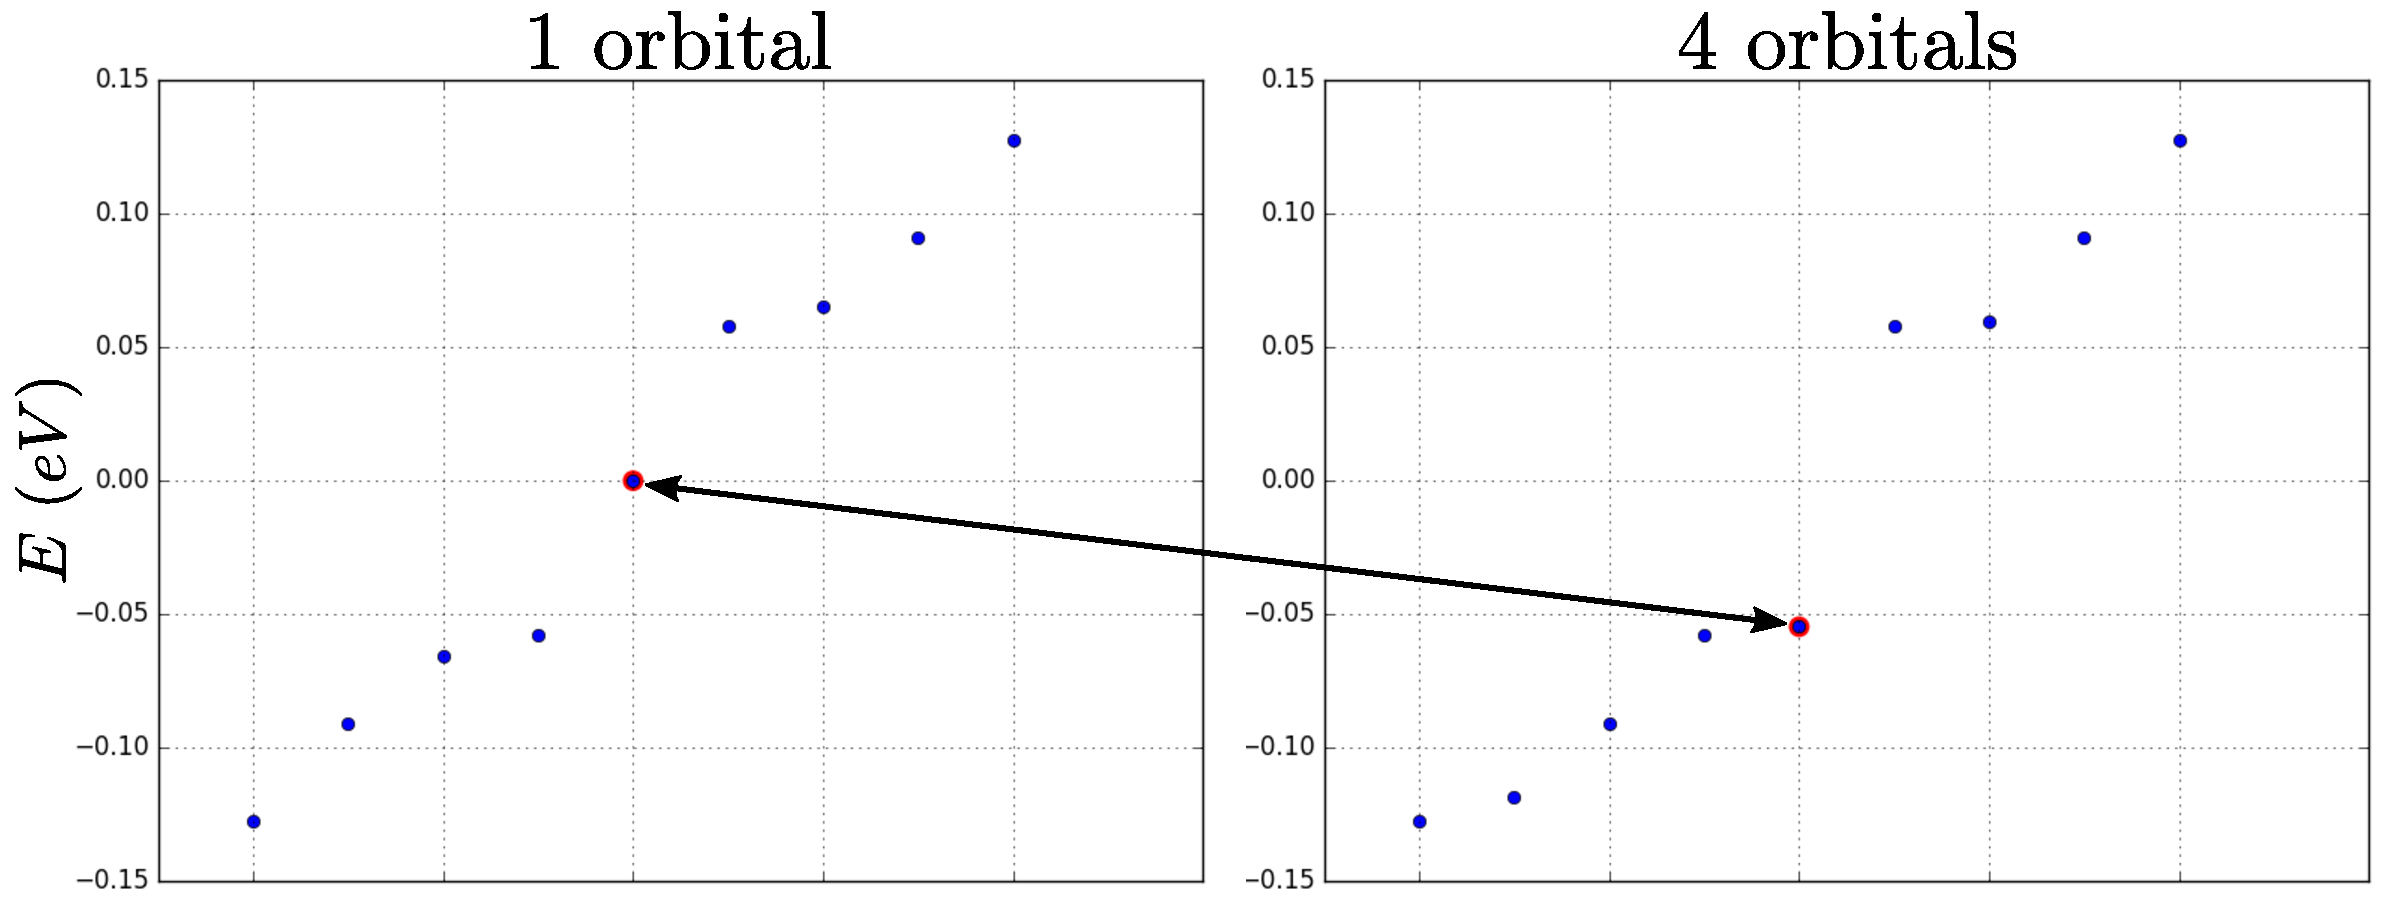
\includegraphics[width=0.8\textwidth]{defects/fig/spectrum.pdf}
%  \vspace{-5pt}
%\caption{Low energy spectrum of an armchair island. Left panel shows the spectrum when only the $p_z$ orbitals are considered. Right panel shows the spectrum considering all 4 orbitals $s$, $p_x$, $p_y$, $p_z$}
%\label{spectrum}
%\end{figure}
%\FloatBarrier
%%~~~~~~~~~~~~~~~~~~~~~~~~~~~~~~~~~~~~~~~~~~~~~~~~~~~~~~~~~~~%
%
%Notice in figure~\ref{spectrum} that the in-gap state, marked in red, does not appear at $E=0$ as this system is no longer suitable for the Lieb's theorem. The exact energy at which the in-gap state appear depends on the hopping parameters between the $H$ and the $C$ atoms, mainly on the $V_{sp\sigma}$ parameter.
%
%
%\red{XXX}


The parameters in \ref{G_SK_params} were calculated for $H$ passivating the edges of graphene nanoribbons\cite{Gosalbez-Martinez2011} where the main hybridization occurs with the $\sigma$ orbitals of graphene. There is no good reason why these hoppings parameters should hold for an adatom, so we can consider the hopping parameters, $V_{ss\sigma}$ and $V_{sp\sigma}$, between the chemisorbed Hydrogen and graphene as somehow free parameters that we can tune.

The energy of the in-gap state as a function of both parameters is shown in \fref{ingap}. Notice the strong dependence with the $V_{sp\sigma}$ parameter.
%~~~~~~~~~~~~~~~~~~~~~~~~~~ FIGURE ~~~~~~~~~~~~~~~~~~~~~~~~~%
\begin{figure}[h!]
  \centering
  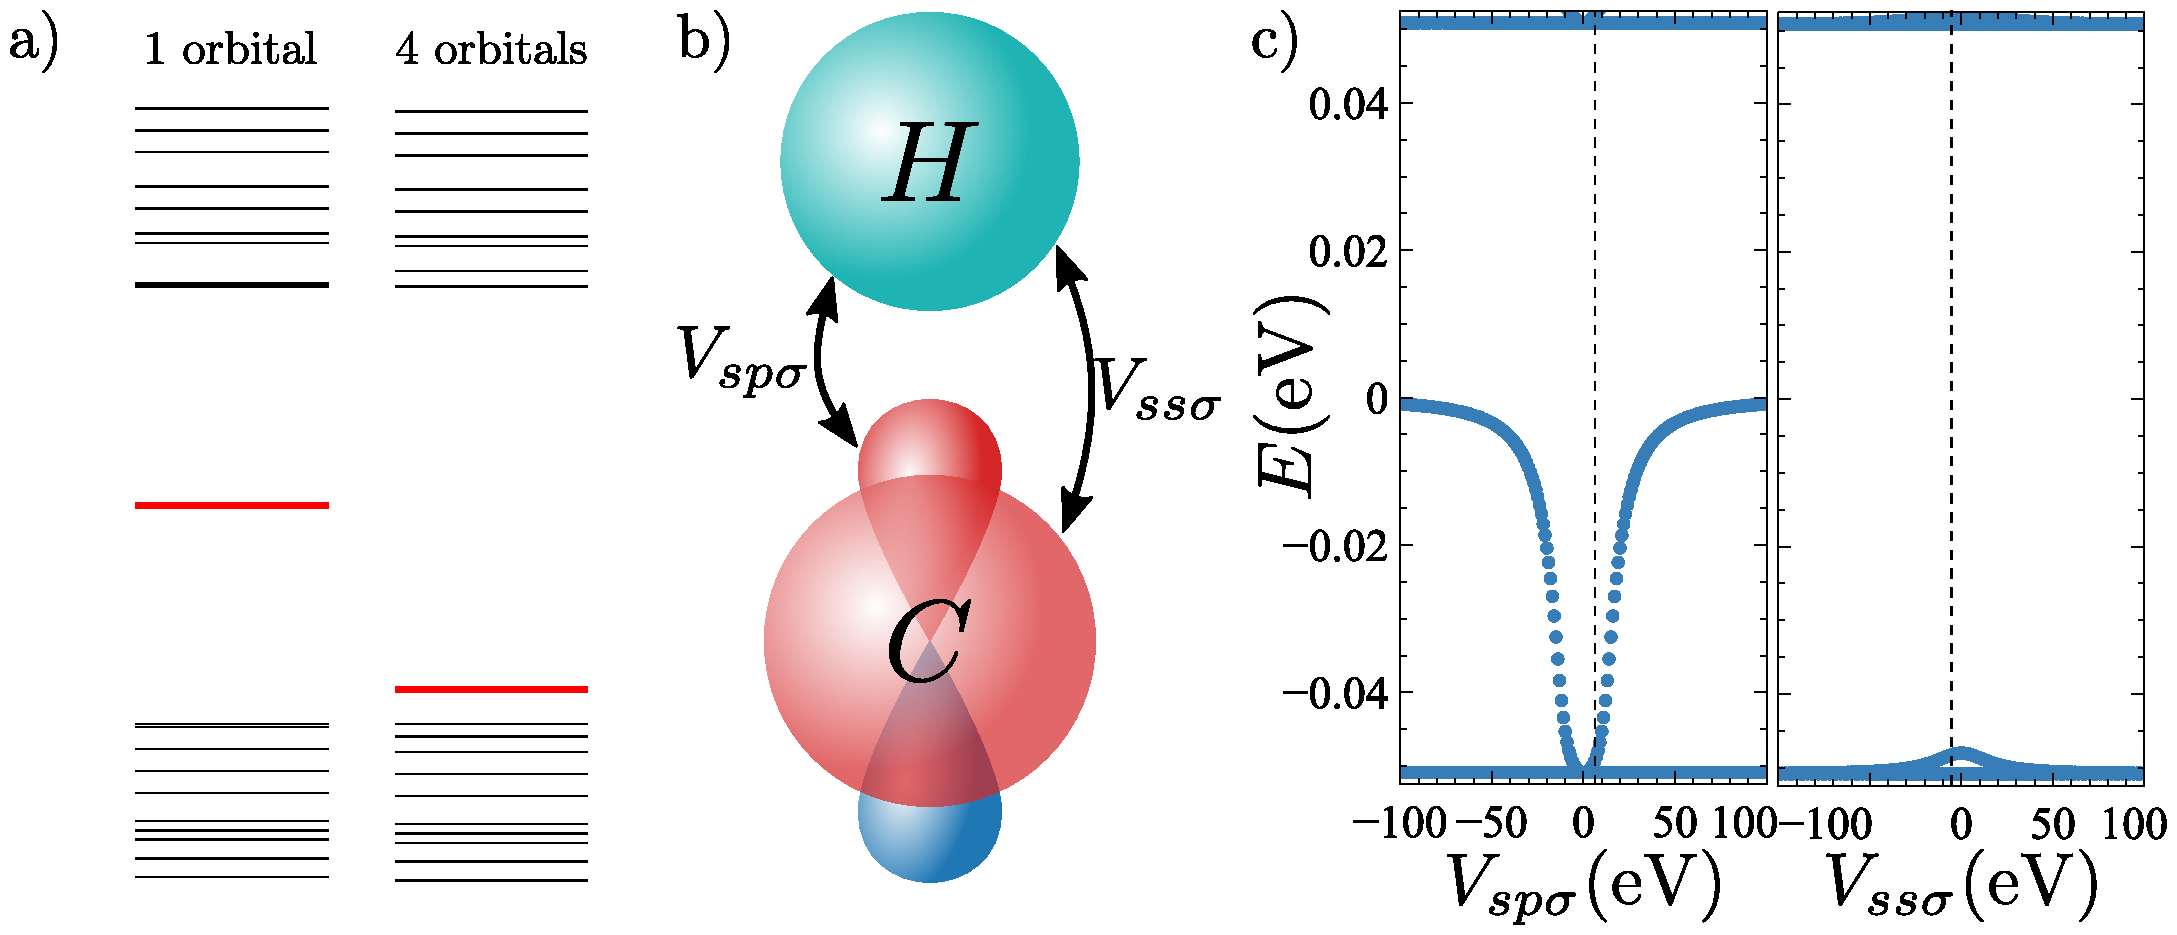
\includegraphics[width=0.8\textwidth]{defects/fig/Vsss_Vsps.pdf}
  \vspace{-5pt}
  \caption{a) Comparison of the spectrum (sketch) of a graphene island using the vacancy in a one orbital model and an adatom in the \ac{sk} approximation using the parameters in \ref{G_SK_params}. Notice that the in-gap state appears close to the valence band rather than in the middle of the gap. b) Scheme of the hopping processes present in this kind of defects. c) 2-D representation of the position of the in-gap state as a function of the \ac{sk} parameters. c) Evolution of the spectrum of an armchair island for different \ac{sk} parameters for the $sp^3$ defect. Notice the strong dependence of the in-gap energy with $V_{sp\sigma}$ especially comparing it with $V_{ss\sigma}$.}
\label{ingap}
\end{figure}
\FloatBarrier
%~~~~~~~~~~~~~~~~~~~~~~~~~~~~~~~~~~~~~~~~~~~~~~~~~~~~~~~~~~~%
It is clear that in order to recover the 1 orbital intuition (in-gap state at $E=0$), we require the limit for $V_{sp\sigma}\to\infty$. The experimental value for these parameters is difficult to infer, so we will consider a wide range of values and explore the resulting physics.

\section{Hyperfine Interaction}
\label{sec:hyperfine}
Apart from the interaction of the electron and the proton with the external magnetic field we have to take into account the interaction between them.

The hyperfine (HF) interaction arises when we consider the effect of the nuclear spin on the electron.

By introducing the potential vector $\vec{A}_{I}$ (corresponding to the magnetic field created by the proton, $\rotac{\vec{A}_{I}}$) in the Hamiltonian and expanding to first order in this potential vector, we get the complete hyperfine Hamiltonian:~\cite{Cohen1977book}
\begin{equation}
H_{hf} = \frac{-\mu_{0}}{4\pi}\left[
\frac{q_{p}}{m_{e}R^{3}}\vec{L}\cdot\vec{M}_{I} +
\frac{1}{R^{3}}\left(3(\vec{m}_{e}\cdot\hat{n})
                      (\vec{m}_{p}\cdot\hat{n})-
                      \vec{m}_{e}\cdot\vec{m}_{p}\right) +
\frac{8\pi}{3}\vec{m}_{e}\cdot\vec{m}_{p}\delta(\vec{R})
\right]
\label{full_HF}
\end{equation}
where $\vec{L}$ is the orbital momentum of the electron, $\vec{m}_{e}$ is the magnetic moment of the electron, and $\hat{n}$ is the unit vector of the straight line joining the proton to the electron.\\

The first term in equation~\eqref{full_HF} represents the interaction of the nuclear magnetic moment with the magnetic field created at the proton by the rotation of the electronic charge. If we are considering $s$ orbitals this term will vanish since all the terms would include a factor like $\bra{n,0,0}L\ket{n,0,0} = 0$, so we will drop this term from the discussion.

The second term represents the dipole-dipole interaction between the nuclear and electronic magnetic moments. Again for a \textit{pure} $s$ orbital this term would vanish as a consequence of the spherical symmetry of the orbital. Nevertheless, because of perturbations (from the crystal or external fields) a contribution from this term may become relevant. \red{review, and check the possible modification of $\mathcal{A}$ due to this geometric deformation}

The third term is the so-called ``contact term'', and arises from the singularity at $\vec{R}=\vec{0}$ of the field created by the magnetic moment of the proton.
This contact term describes the interaction of the magnetic moment of the electron spin with the magnetic field inside the proton (considered as punctual). Notice that because of the presence of the delta function in this term, it will be proportional to the overlap of the wave function of the electron and the proton. This term will by the main contribution to the hyperfine interaction.\\

For the case of a free, isolated Hydrogen and for the $1s$ orbital the calculation of the contact term can be done exactly:
\begin{equation}
H^{contact}_{hf} =
%\underbrace{\frac{-\mu_{0}}{4\pi}\frac{8\pi}{3}\frac{g_{p}\mu_{n}}{\hbar}
%\frac{g_{e}\mu_{e}}{\hbar}}_{\mathcal{A}_{0}} \vec{I}\vec{S}
\frac{-2\mu_0}{3}\frac{g_{p}\mu_{n}}{2}
\frac{g_{e}\mu_{e}}{2} \bra{1,0,0}\delta(\vec{R})
\ket{1,0,0}  \vec{\sigma}_e\vec{\sigma}_p =
\mathcal{A}_{0}\vec{\sigma}_e\vec{\sigma}_p
\end{equation}
where the notation for the kets is $\ket{n,l,m_{l}}$, with $n$ the so-called principal quantum number, $l$ the orbital angular momentum and $m $the third component of said angular momentum. The hyperfine coupling, $\mathcal{A}_{0}$, takes the value \red{(Units done in the last appendix, check)}: %XXX
\begin{equation}
\frac{\mathcal{A}_{0}\hbar}{2\pi} \simeq \SI{1420}{\MHz}
\end{equation}
%XXX
correct?:
\begin{equation}
\frac{4\pi\mathcal{A}_{0}}{\hbar} \simeq \SI{1420}{\MHz}
\end{equation}
bien definitivo (check appendix~\ref{units_A}):
\begin{equation}
  \frac{\mathcal{A}}{2\pi\hbar} = \SI{1420}{\MHz}
\end{equation}

Notice that the contribution to the hyperfine contact term for $p$ (or higher $l$) orbitals vanishes since the wave functions of such orbitals vanish at the nucleus position, so the factor $\bra{n,l,m_{l}}\delta(\vec{R})\ket{n,l,m_{l}}$ will always be zero.\\

In general, the effective hyperfine coupling of a given state will be considered proportional to the weight of the wave function on the Hydrogen $s$ orbital.

\begin{equation}
  \mathcal{A} = A_0|\braket{\phi_s}{\psi}|^2
\end{equation}

Of course other orbitals centered at the other atoms would also contribute to the hyperfine interaction (since the wave function does not vanish at the position of the nucleus), nevertheless the \ac{tb} approximation does not offer the tools to deal with the deformation of the orbitals what makes it impossible to estimate the evaluation of the orbitals at the $H$ nucleus and comparison with \ac{dft} calculations show that this effect is not the main one for describing this physics.

For the case of Si:$^{31}$P the hyperfine coupling in MegaHertz is $4\pi\mathcal{A}/\hbar=58MHz$
\red{check factor}



%~~~~~~~~~~~~~~~~~~~~~~~~~~ FIGURE ~~~~~~~~~~~~~~~~~~~~~~~~~%
\begin{figure}[h!]
\centering
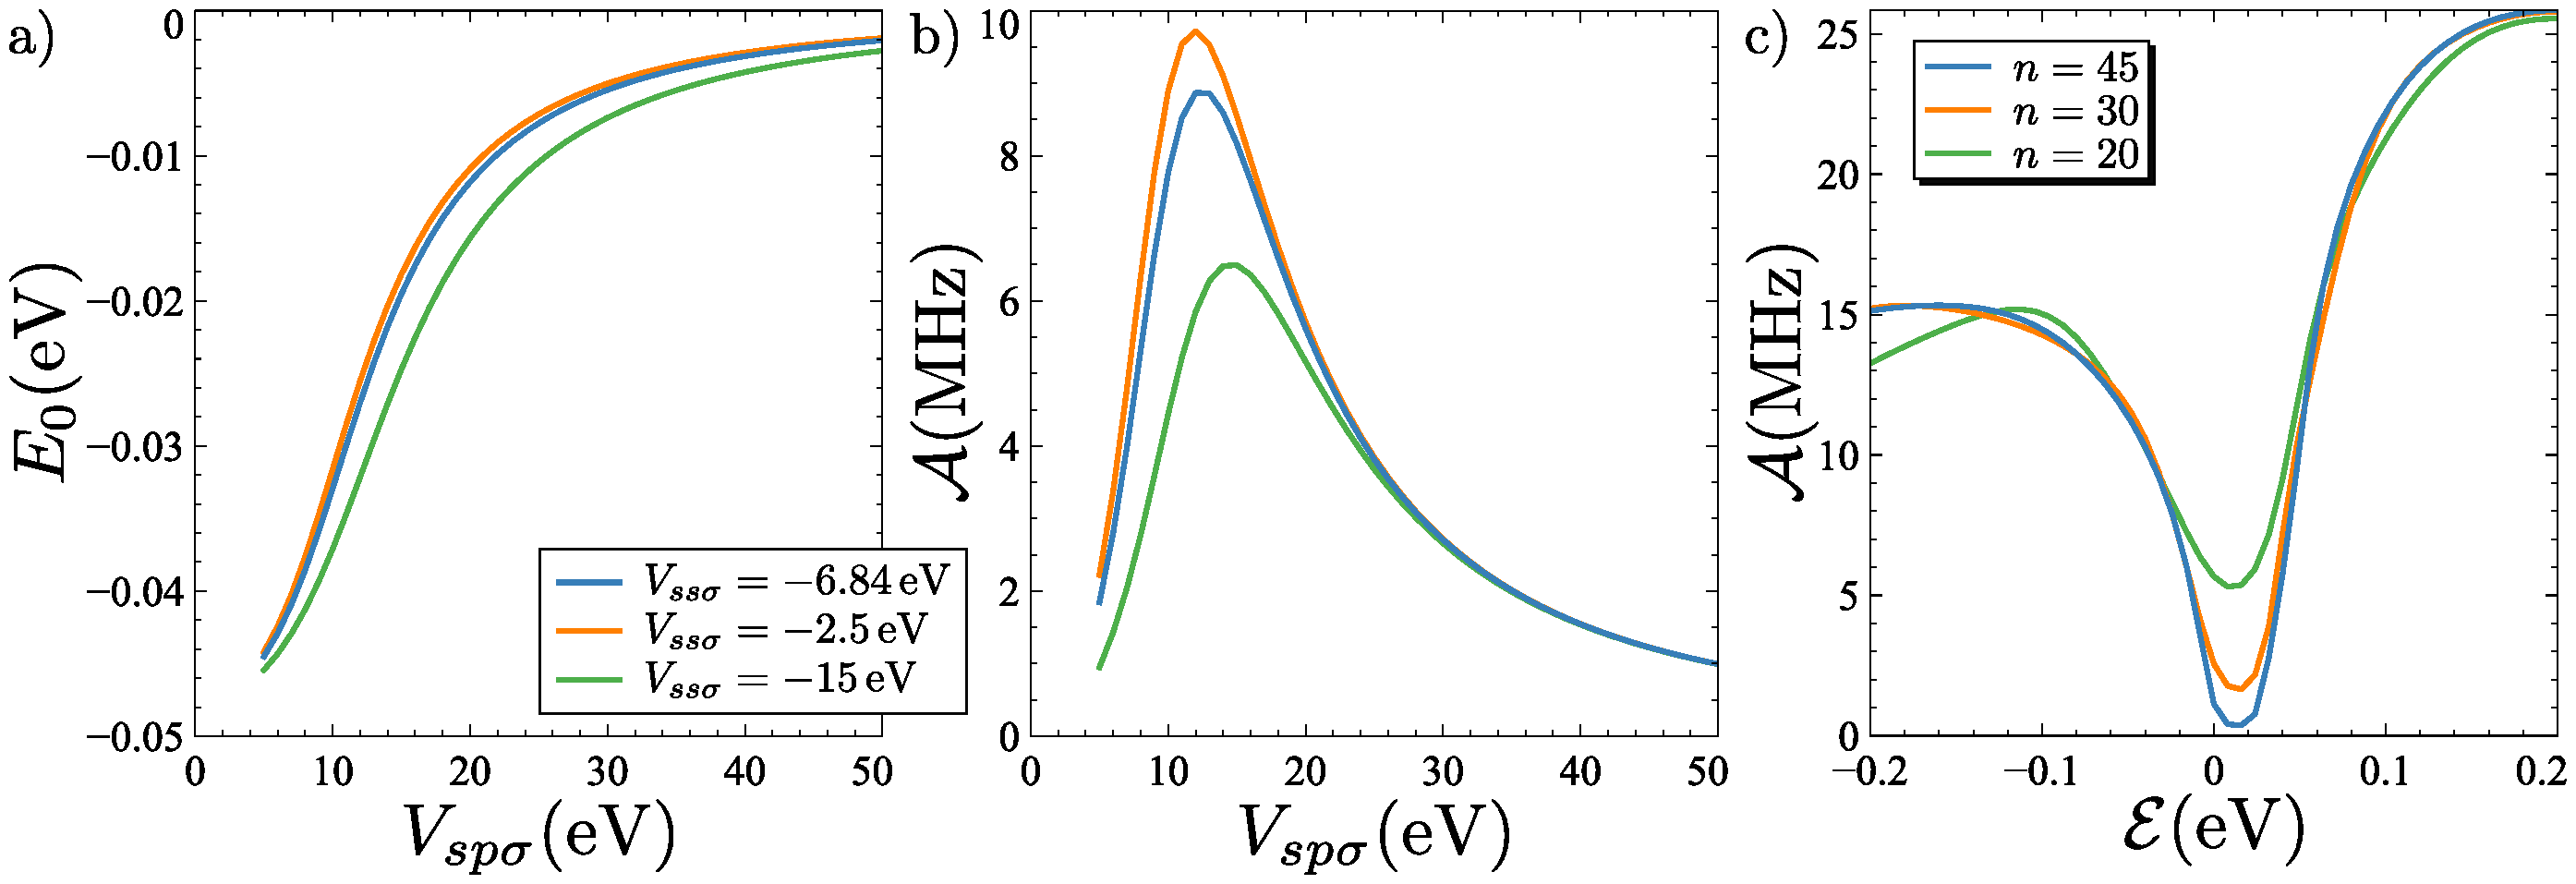
\includegraphics{defects/fig/coupling_hyper.pdf}
\vspace{-10pt}
\caption{a) Dependence of the in-gap state arising from a single vacancy in graphene monolayer with the $V_{sp\sigma}$ coupling for different $V_{ss\sigma}$. b) Hyperfine coupling with the $V_{sp\sigma}$ coupling in a H adatom on top of graphene.} % c) Hyperfine coupling modulated by an external electric field in bilayer graphene calculated with the optimal parameters calculated in the monolayer case. These numbers are to be considered as an upper limit for the tunability of $\mathcal{A}$.}
\label{hyperfine}
\end{figure}
\FloatBarrier
%~~~~~~~~~~~~~~~~~~~~~~~~~~~~~~~~~~~~~~~~~~~~~~~~~~~~~~~~~~~%




\subsection{A Qubit Idea}


Finally, we can write the complete Hamiltonian for our nuclear qubit as a combination of the previous ones:
\begin{equation}
  H = -g_e\mu_e\frac{1}{2}\vec{B}\vec{\sigma}^e
      -g_p\mu_p\frac{1}{2}\vec{B}\vec{\sigma}^p
      +A\vec{\sigma}^e\cdot\vec{\sigma}^p
\label{1qubit}
\end{equation}
First of all, we can make a quick estimation of the order of magnitude of each of these terms:
\begin{itemize}
  \item Zeeman for the electron: $g_e\mu_e\simeq\SI{-115.9}{\micro\eV\per\tesla}$
  % -2\cdot5.79\cdot10^{-5}\simeq-1.16\cdot10^{-4}eV/T$
  \item Zeeman for the proton: $g_p\mu_p\simeq\SI{0.176}{\micro\eV\per\tesla}$
  % 5.6\cdot3.15\cdot10^{-8}\simeq1.7\cdot10^{-7}eV/T$
  \item Hyperfine: Assuming
  $\mathcal{A}=58MHz\Rightarrow\mathcal{A}\simeq\SI{0.003}{\micro\eV}$
% 6.6\cdot10^{-08}eV$
\end{itemize}
We are stretching a bit the notation in the Hamiltonian \eqref{1qubit} since each of the terms is expressed in a different basis. Namely, each of the Zeeman terms act only in the electron \textbf{or} proton spin subspace but the hyperfine coupling has to be expressed in a 2-particle basis that have not been defined yet.
To fix the notation we define the following 2-particle basis:
\begin{equation}
  \mathcal{B}=\left\{\ket{\up\up},\ket{\up\down},
                     \ket{\down\up},\ket{\down\down}\right\}
\label{basis}
\end{equation}
% where the simple arrows $\uaw\daw$ represent the $S_z$ eigenvectors of the electronic spin, and the double arrows $\Uaw\Daw$ represent the $S_z$ eigenvectors of the nuclear spin.
where the first position of the ket corresponds to the electronic state and the second to the nuclear one.

In this basis the Pauli matrices are expressed as follows.
\begin{equation}
  \begin{split}
    \sigma^e_x=\left(\begin{array}{cccc}
    0 & 0 & 1 & 0 \\
    0 & 0 & 0 & 1 \\
    1 & 0 & 0 & 0 \\
    0 & 1 & 0 & 0
    \end{array}\right)\quad;\quad
    \sigma^e_y=\left(\begin{array}{cccc}
    0 & 0 & -i & 0 \\
    0 & 0 & 0 & -i \\
    i & 0 & 0 & 0 \\
    0 & i & 0 & 0
    \end{array}\right)\quad;\quad
    \sigma^e_z=\left(\begin{array}{cccc}
    1 & 0 & 0 & 0 \\
    0 & 1 & 0 & 0 \\
    0 & 0 & -1 & 0 \\
    0 & 0 & 0 & -1
    \end{array}\right)\\
    \sigma^p_x=\left(\begin{array}{cccc}
    0 & 1 & 0 & 0 \\
    1 & 0 & 0 & 0 \\
    0 & 0 & 0 & 1 \\
    0 & 0 & 1 & 0
    \end{array}\right)\quad;\quad
    \sigma^p_y=\left(\begin{array}{cccc}
    0 & -i & 0 & 0 \\
    i & 0 & 0 & 0 \\
    0 & 0 & 0 & -i \\
    0 & 0 & i & 0
    \end{array}\right)\quad;\quad
    \sigma^e_z=\left(\begin{array}{cccc}
    1 & 0 & 0 & 0 \\
    0 & -1 & 0 & 0 \\
    0 & 0 & 1 & 0 \\
    0 & 0 & 0 & -1
    \end{array}\right)
  \end{split}
\end{equation}
Hence, our Hamiltonian for two qubits in the presence of an off-plane magnetic field, $\vec{B}=(0,0,B/2)$, can be expressed as follows:
\begin{equation*}
H = \underbrace{-g_e\mu_e\frac{1}{4}}_{E}B\sigma^e_z
    \underbrace{-g_p\mu_p\frac{1}{4}}_{P}B\sigma^p_z
    +A\vec{\sigma}^e\cdot\vec{\sigma}^p
\end{equation*}
\begin{equation}
  H = \left(\begin{array}{cccc}
  B(E+P)+A & 0 & 0 & 0 \\
  0 & B(E-P)-A & 2A & 0 \\
  0 & 2A & B(-E+P)+A & 0 \\
  0 & 0 & 0 & B(-E-P)-A
  \end{array}\right)
\end{equation}

The eigenvalues of this matrix are the following \red{irrelevant?}:
\begin{equation}
  \begin{split}
    E_0 &= -A-B(P+E) \quad;\quad v_0=\left(0,0,0,1\right)\\
    E_1 &= A+B(P+E) \quad;\quad v_1=\left(1,0,0,0\right)\\
    E_2 &= -\sqrt{A(5A+2B(P-E)) + B^2 (P-E)^2} \\
        &\quad\quad\quad\quad v_2 =\left(0,-\frac{A+B(P-E)+\sqrt{A(5A+2B(P-E)) + B^2 (P-E)^2}}{2 A},1,0\right)\\
    \quad\\
    E_3 &= \sqrt{A(5A+2B(P-E)) + B^2 (P-E)^2}\\
        &\quad\quad\quad\quad v_3 = \left(0,-\frac{A+B(P-E)-\sqrt{A(5A+2B(P-E)) + B^2 (P-E)^2}}{2 A},1,0\right)
  \end{split}
\label{eig}
\end{equation}



For now we will neglect the contribution of the proton and check the behavior of the eigenenergies of the system as a function of both the external magnetic field and the hyperfine coupling.
%~~~~~~~~~~~~~~~~~~~~~~~~~~ FIGURE ~~~~~~~~~~~~~~~~~~~~~~~~~%
%TODO make this picture nicer
\begin{figure}[h!]
\centering
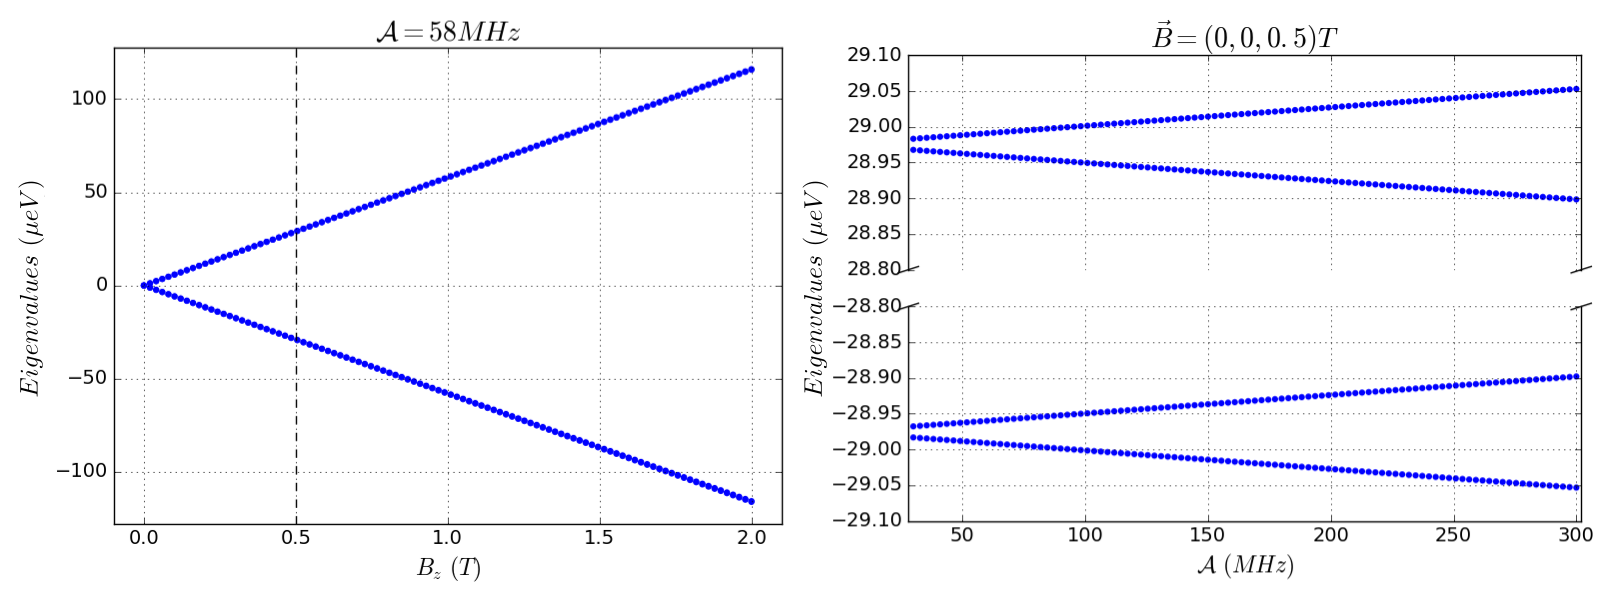
\includegraphics[width=0.9\textwidth]{chapter03/figures/spectrum.png}
\vspace{-5pt}
\caption{Evolution of the eigenvalues of the Hamiltonian \eqref{1qubit} with the magnetic field, $B$, and the hyperfine interaction, $\mathcal{A}$. The dashed line is used to indicate the magnetic field in the second figure}
\label{spectrum}
\end{figure}
\FloatBarrier
%~~~~~~~~~~~~~~~~~~~~~~~~~~~~~~~~~~~~~~~~~~~~~~~~~~~~~~~~~~~%
In figure~\ref{spectrum} we can see that the energy levels are separated in two sets split by the electronic Zeeman splitting (remember that we are neglecting the proton Zeeman coupling here). The splitting within each of these sets is governed by the hyperfine coupling.

But as we said before, the hyperfine coupling and Zeeman coupling for the proton are in the same order of magnitude. When we include the proton Zeeman interaction the big picture is the same: two sets of levels split by the electronic Zeeman. But within each of these two sets there is a difference, depending on the magnitude of the magnetic field and the hyperfine coupling the ordering of the wave functions may change. \red{rephrase}
%~~~~~~~~~~~~~~~~~~~~~~~~~~ FIGURE ~~~~~~~~~~~~~~~~~~~~~~~~~%
\begin{figure}[h!]
\centering
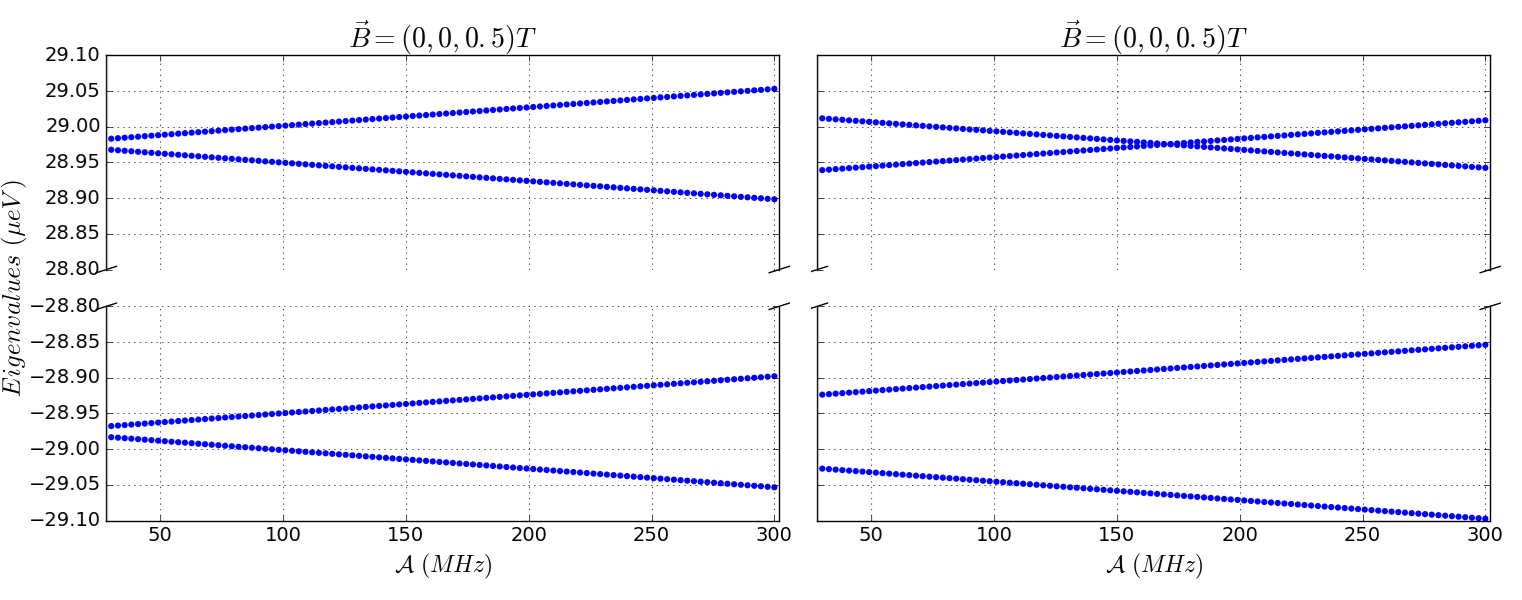
\includegraphics[width=0.9\textwidth]{chapter03/figures/pro_nopro.png}
\vspace{-5pt}
\renewcommand{\figurename}{\footnotesize{\textsc{Figure}}}
\caption{Comparison of the energy levels as a function of the hyperfine coupling. Panel $a)$ neglects the Zeeman term for the proton, in panel $b)$ we use the full Hamiltonian. (Both panels share the $Y$ axis)}
\label{proton}
\end{figure}
\FloatBarrier
%~~~~~~~~~~~~~~~~~~~~~~~~~~~~~~~~~~~~~~~~~~~~~~~~~~~~~~~~~~~%
The level crossing that appears in figure~\ref{proton} represents nothing more than the exchange of the wave functions as it can be seen in the analytical expression~\eqref{eig}. In fact using these expressions we can get the expression for this level crossing:
\begin{equation}
  \mathcal{A}_{\times}=\frac{B}{2}\left(E\pm\sqrt{E^2+4EP}\right)
\end{equation}


To clarify the meaning of this spectrum we make a schematic representation of the eigenfunctions, shown in figure~\ref{levels1Qbit}. The left column in the table represents the wave functions neglecting the proton's Zeeman contribution. The two columns in the right do not neglect the proton's coupling, and show the cases of high magnetic field (or low hyperfine coupling) and low magnetic field (or high hyperfine coupling). It is clear that depending on the relative magnitude of the proton's Zeeman effect and the Hyperfine coupling the order of the wave functions may differ.
%~~~~~~~~~~~~~~~~~~~~~~~~~~ FIGURE ~~~~~~~~~~~~~~~~~~~~~~~~~%
%TODO 0.004 ueV/T add "/T" in the picture. Qbit notation arrow ---> 0/1
\begin{figure}[h!]
\centering
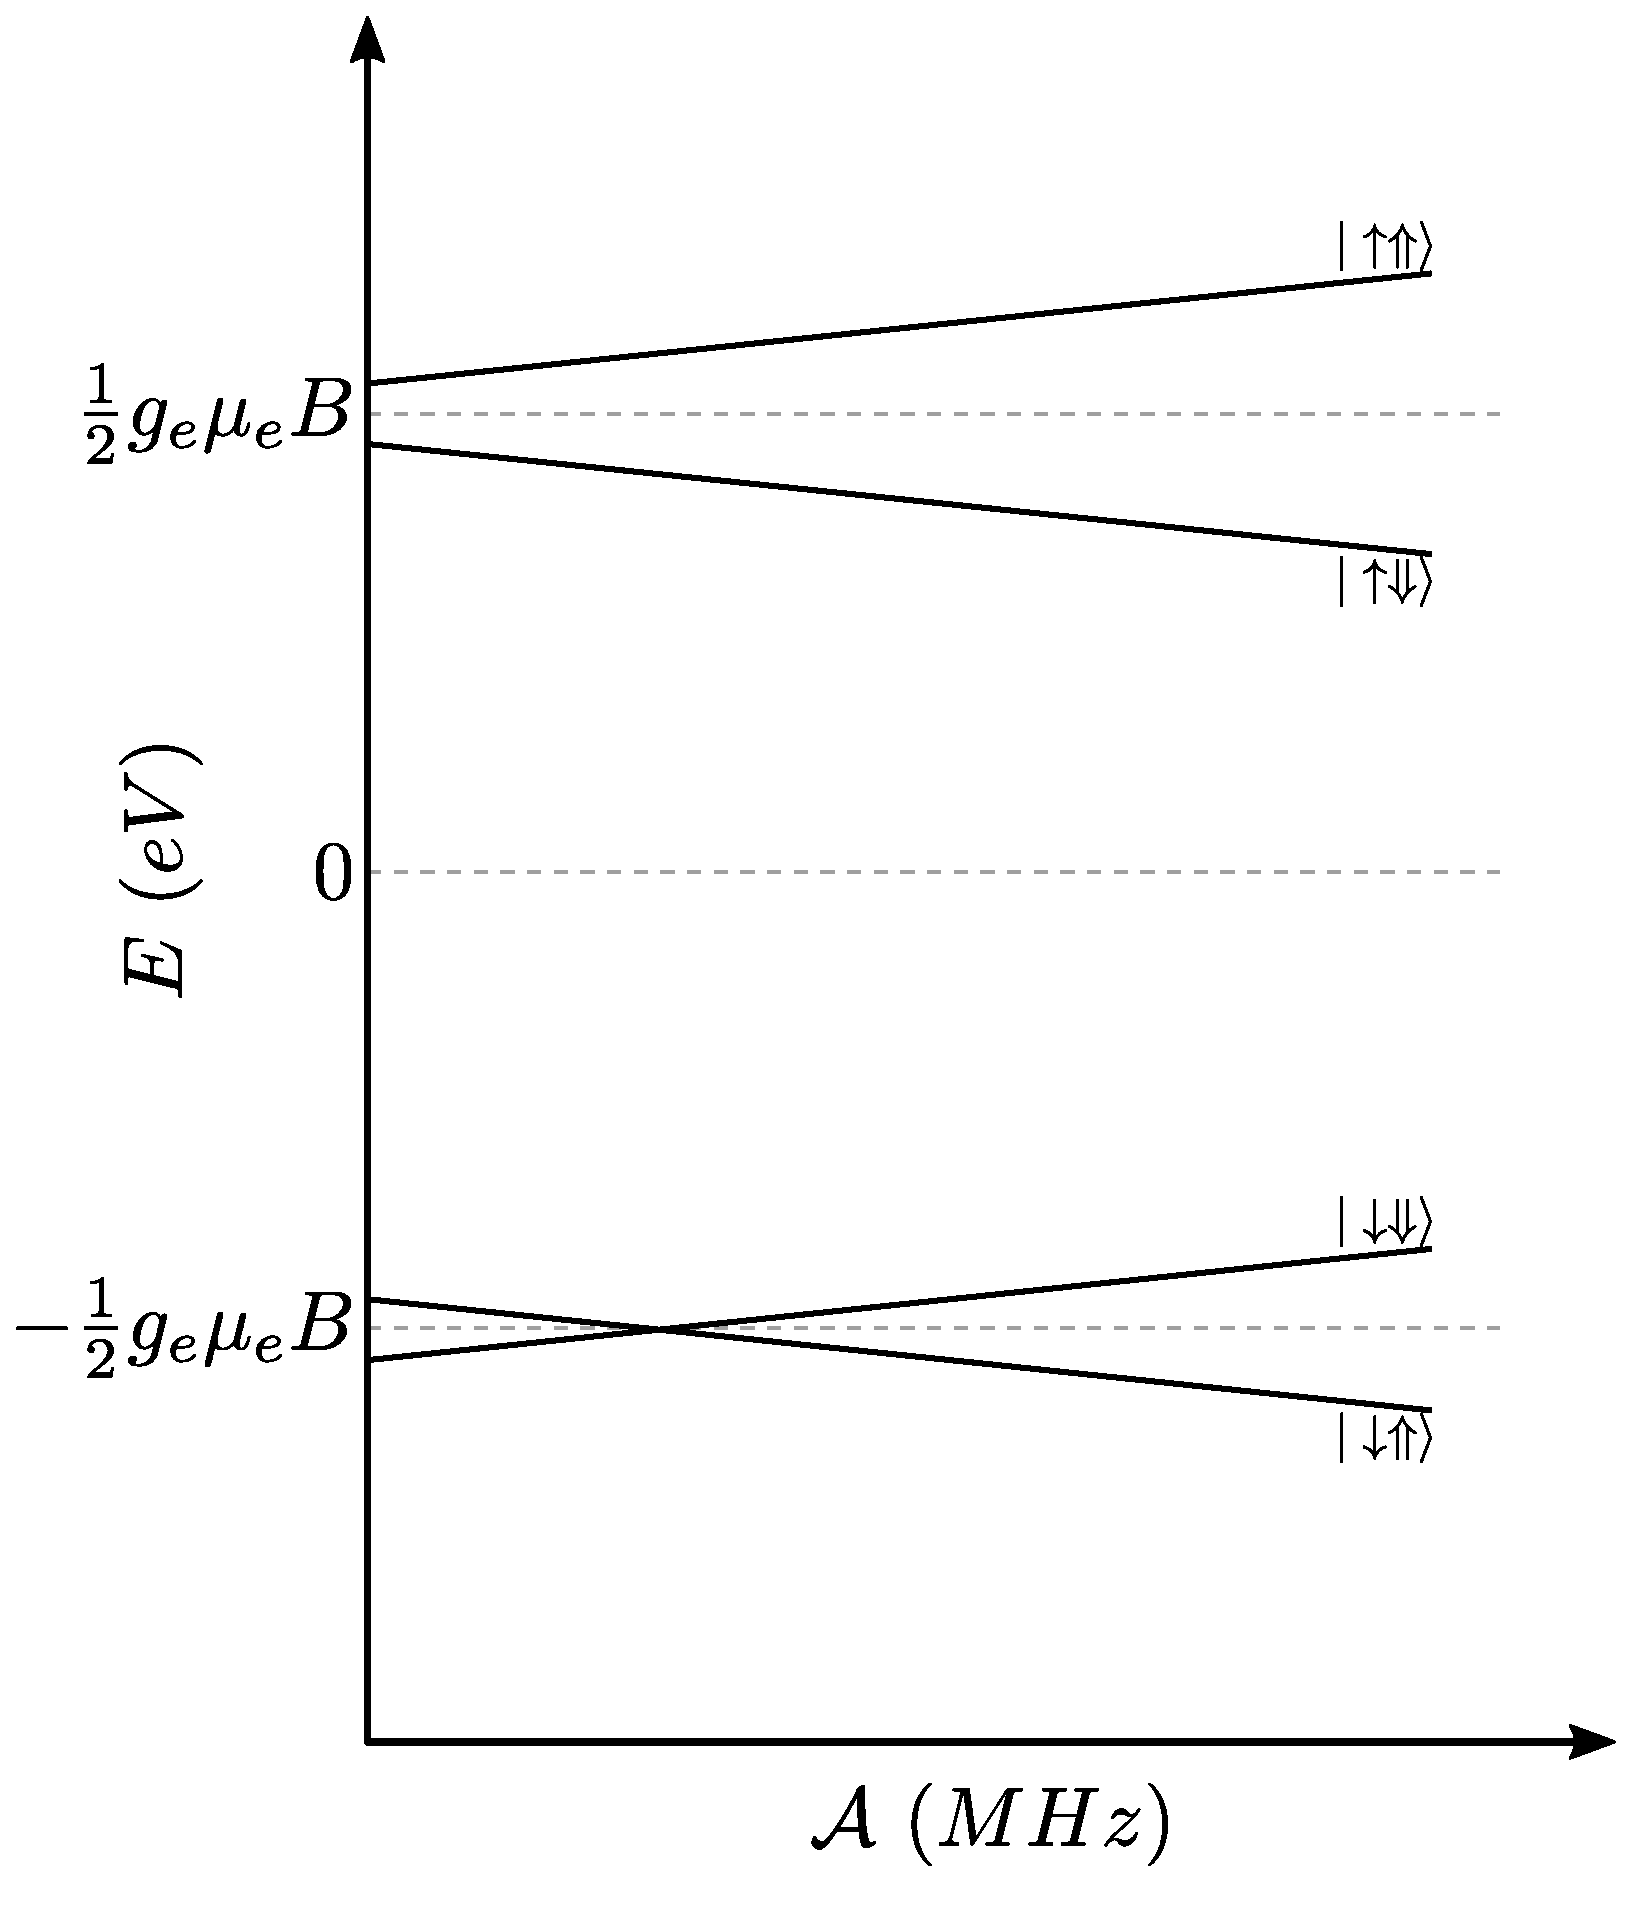
\includegraphics{chapter03/figures/levels1Qbit.pdf} %levels.png}
\vspace{-5pt}
\caption{Sketch of the energy levels for the 1 Qubit Hamiltonian~\eqref{1qubit}. The main splitting among the different states is mainly due to the electronic Zeeman terms. The lowest energy state is determined by the competition between the nuclear Zeeman splitting and the hyperfine interaction.}
% \caption{Schematic representation of the energy levels and its respective wave functions. The states $\ket{\daw\Uaw}$ and $\ket{\uaw\Daw}$ and in fact mixed, but it is negligible (this means that $\ket{\uaw\Daw}\simeq0.9999999\ket{\uaw\Daw}+0.0002672\ket{\daw\Uaw}$). All the possible transitions are specified by $\delta_i$.}
\label{levels1Qbit}
\end{figure}
\FloatBarrier
%~~~~~~~~~~~~~~~~~~~~~~~~~~~~~~~~~~~~~~~~~~~~~~~~~~~~~~~~~~~%
% The states $\ket{\daw\Uaw}$ and $\ket{\uaw\Daw}$ do not in fact appear with weight 1, instead there is a small mixing (less than $0.001\%$).
%
% \red{I think the order of my states is not exactly the same as Morello's. Check}
% Notice that $\delta_1$ and $\delta_2$ will be quite similar ($\SI{50}{\eV/\tesla}$) and $\delta_3$, $\delta_4$ will also be very similar ($\SI{0.05}{\eV/\tesla}$). These frequencies correspond to the energy necessary for flipping respectively the electron spin and the nuclear spin.
%
% \red{Nuclear magnetic resonance and stuff}






% We start by plotting the position of the in-gap state and the hyperfine coupling  as a function of the two parameters
% 
% 
% %~~~~~~~~~~~~~~~~~~~~~~~~~~ FIGURE ~~~~~~~~~~~~~~~~~~~~~~~~~%
% \begin{figure}[h!]
%   \centering
%   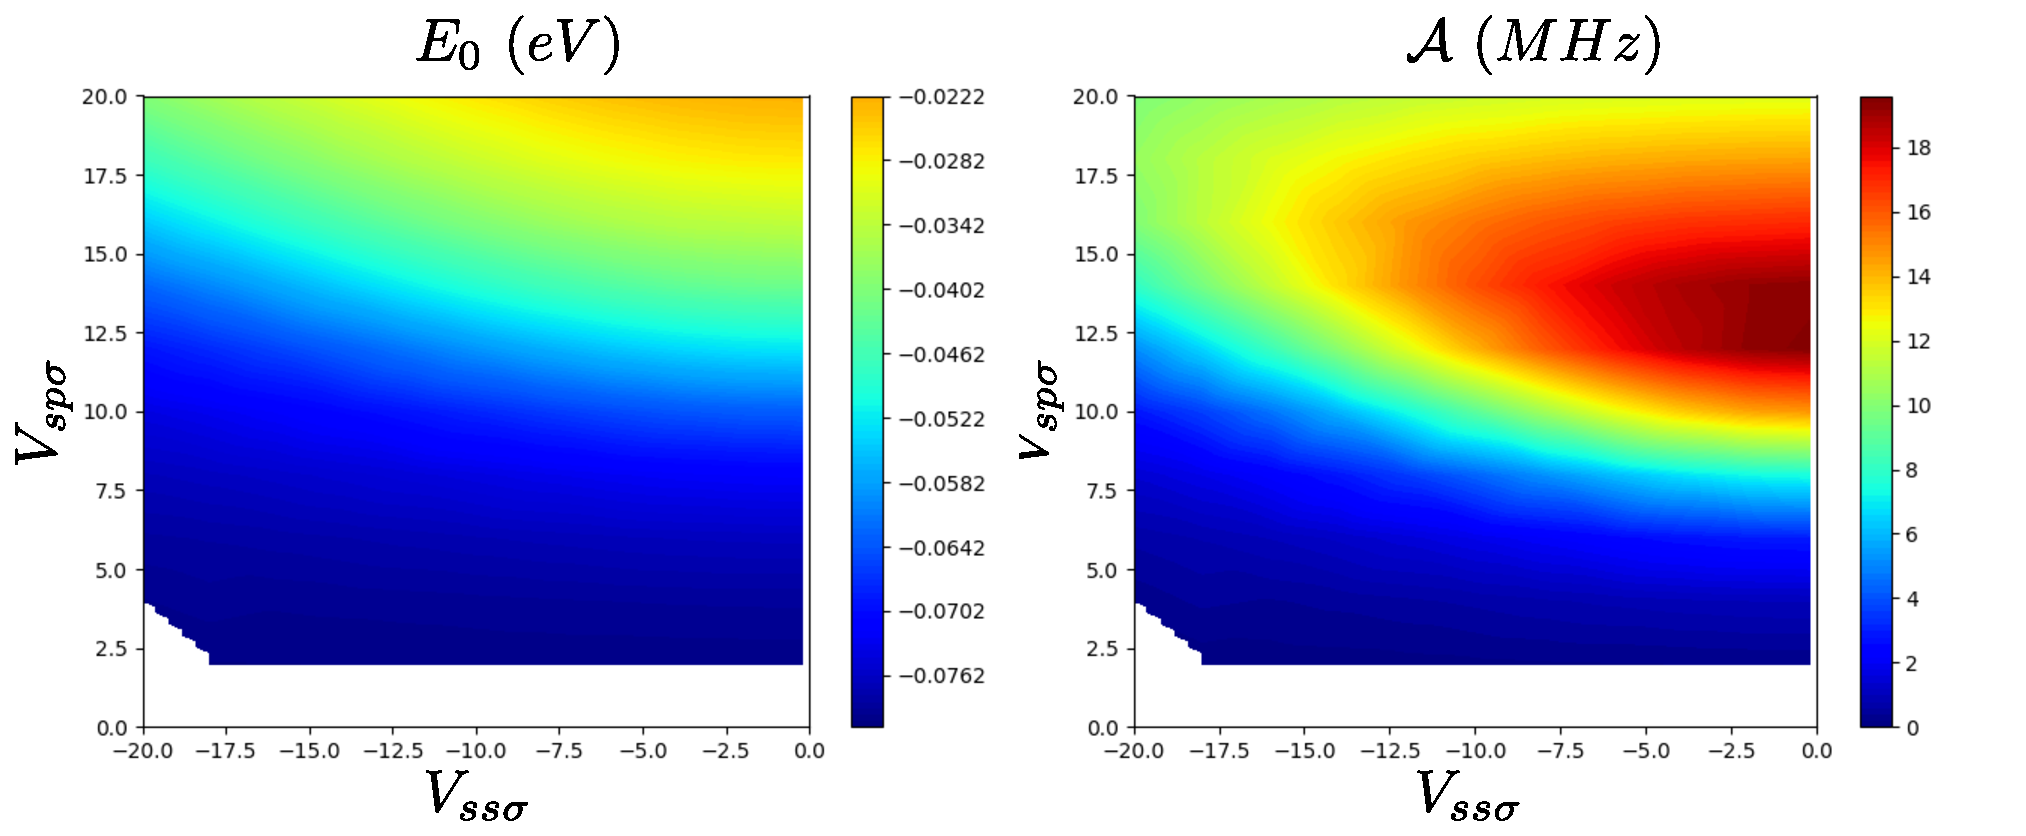
\includegraphics[width=0.9\textwidth]{defects/fig/parameter_space_mono.pdf}
%   \vspace{-5pt}
% \caption{Parameter space for the energy of the in-gap state and the hyperfine coupling for a graphene nanoisland.}
% \label{SK2d}
% \end{figure}
% \FloatBarrier
% %~~~~~~~~~~~~~~~~~~~~~~~~~~~~~~~~~~~~~~~~~~~~~~~~~~~~~~~~~~~%
% 
% 
% 
% 
% 
% 
% 
% \section{Graphene bilayer}
% Graphene bilayer can be described in a analogously. The interlayer hopping is estimated by scaling down the parameters \eqref{SK_params} by a factor, $\xi$, such that the $p_z-p_z$ interlayer hopping takes a value\cite{KatsnelsonBook} of $\xi t_{p_z-p_z}\simeq 0.4eV$.
% % Fig~\ref{hoppings} shows all the possible hoppings between two C atoms in different layers. It is important to notice that in the case of graphene bilayer, the $p_z$ manifold is no longer decoupled from the rest of the orbitals as in the case of graphene.
% % %~~~~~~~~~~~~~~~~~~~~~~~~~~ FIGURE ~~~~~~~~~~~~~~~~~~~~~~~~~%
% % \begin{figure}[h!]
% % \centering
% %   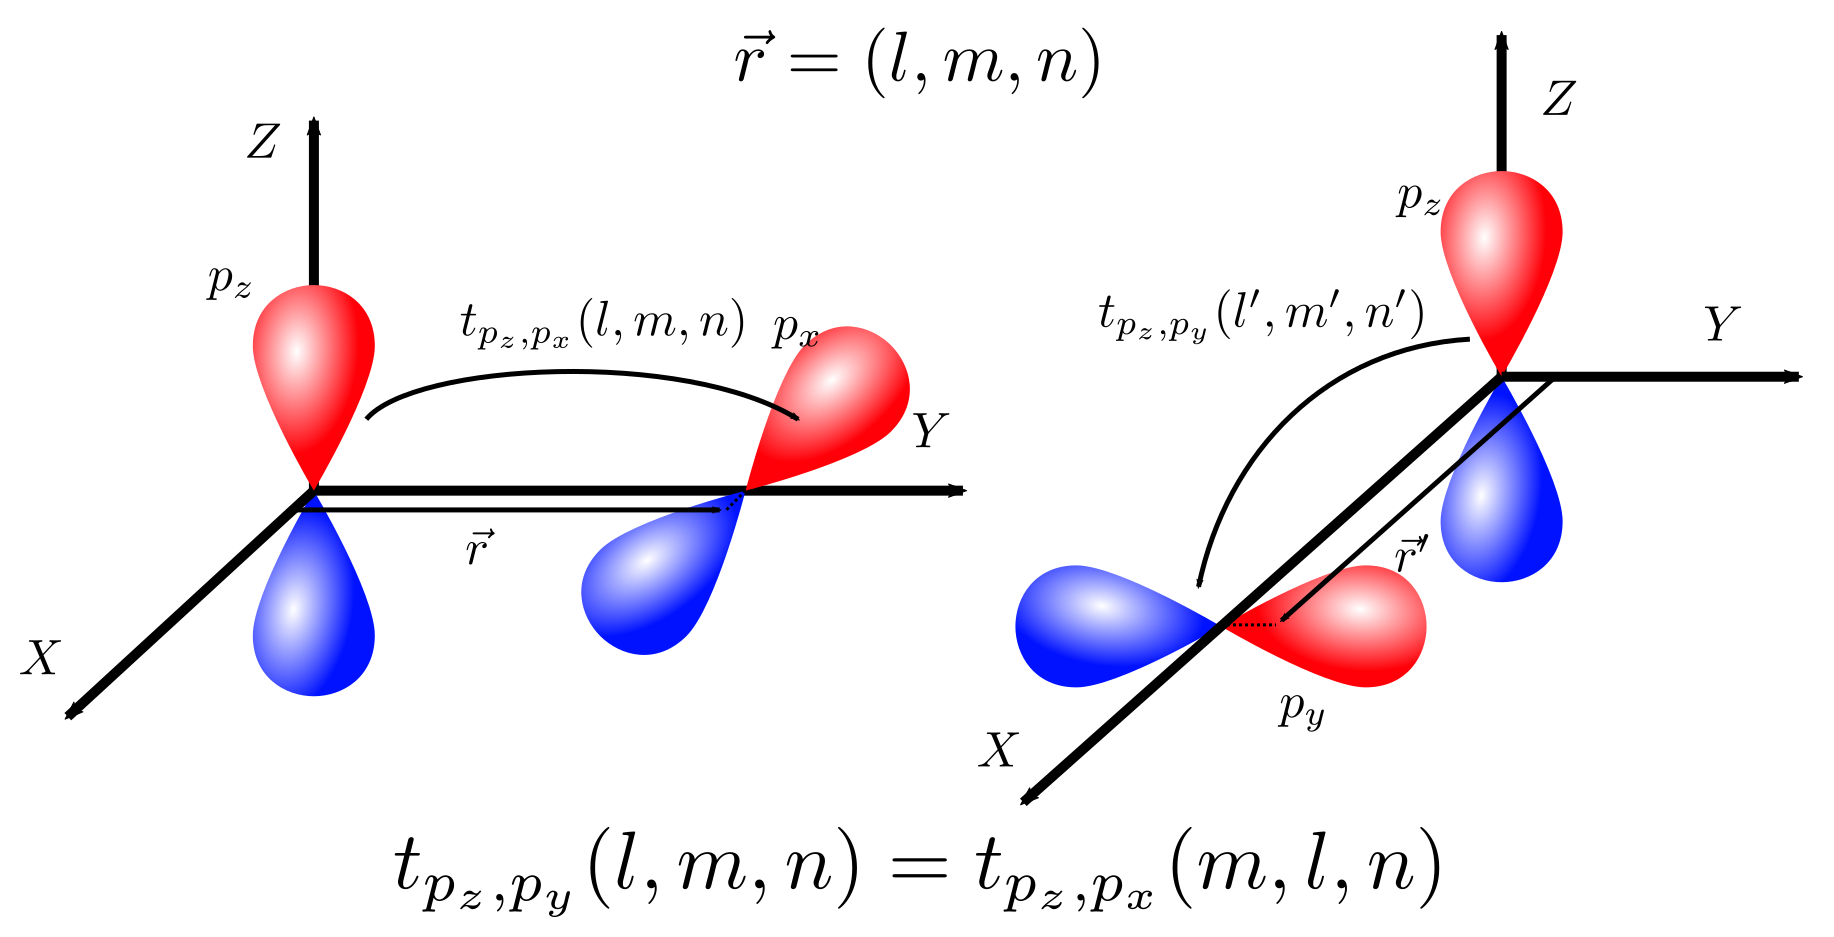
\includegraphics[width=0.45\textwidth]{SK.pdf}
% %   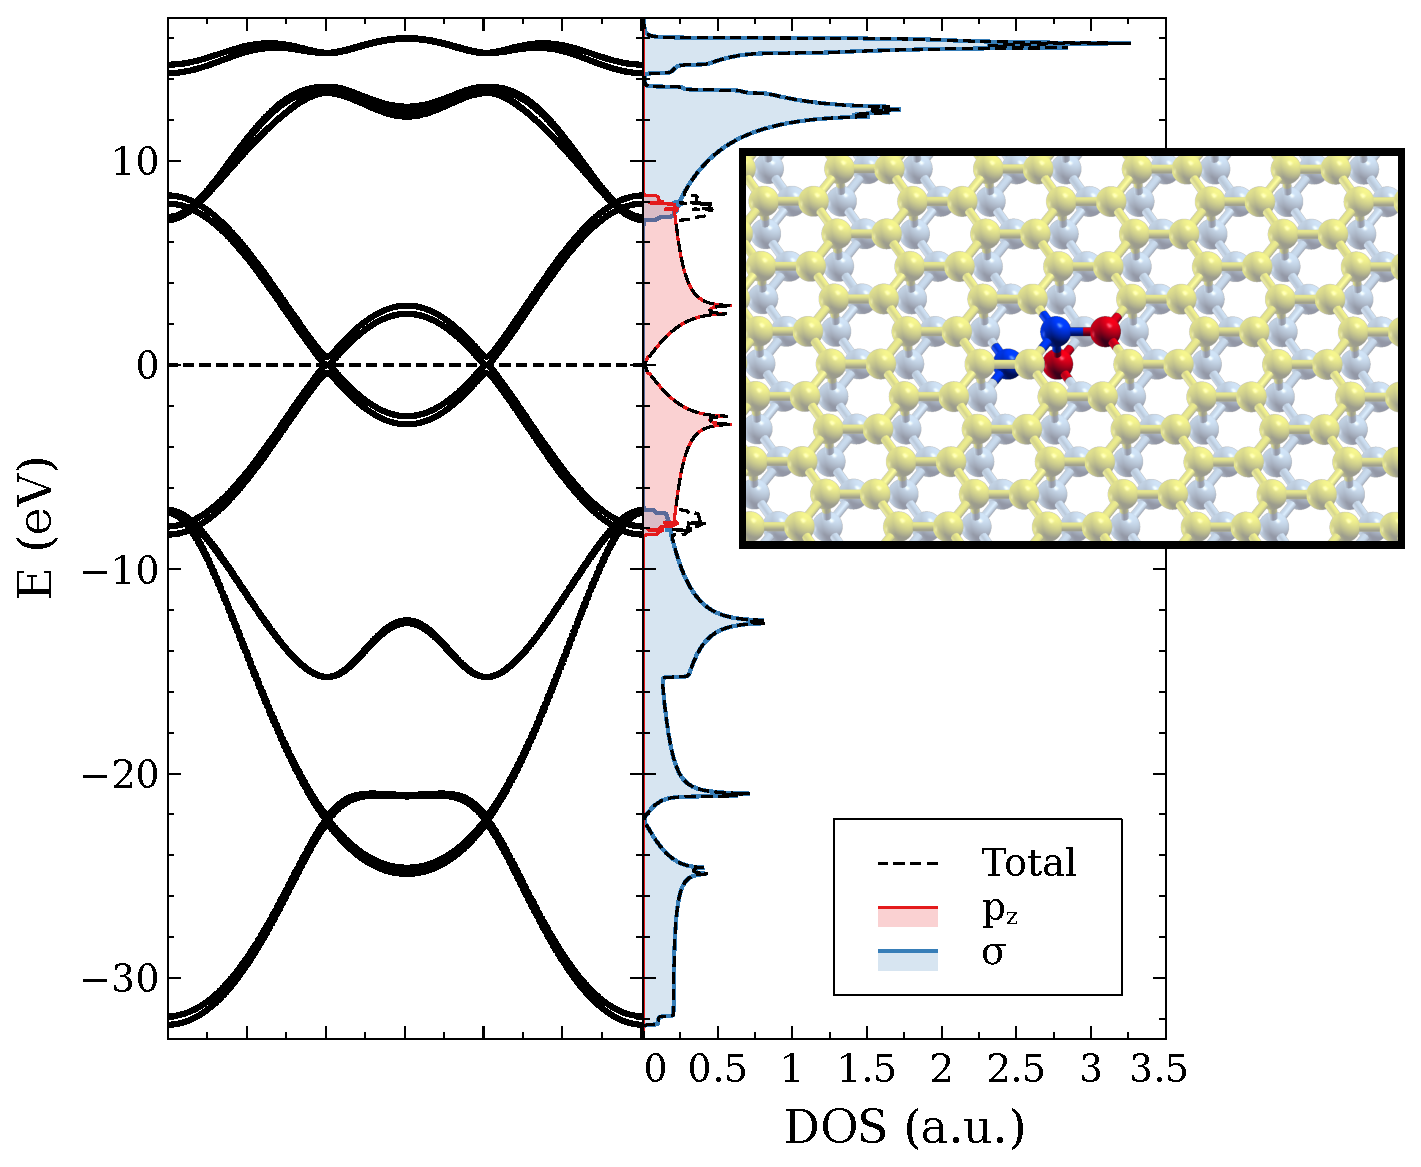
\includegraphics[width=0.45\textwidth]{bilayer_bandDOS.pdf}
% % \vspace{-5pt}
% % \caption{a) Panel show All the possible interlayer hoppings in graphene bilayer. b) Band structure and density of states of graphene bilayer}
% % \label{hoppings}
% % \end{figure}
% % \FloatBarrier
% % %~~~~~~~~~~~~~~~~~~~~~~~~~~~~~~~~~~~~~~~~~~~~~~~~~~~~~~~~~~~%
% \subsection{Electric field}
% % The band structure of graphene bilayer in such a model is shown in \ref{hoppings}.
% The effect of an electric, $\Delta_E$ is to shift the energies of all the orbitals by an amount $\pm\Delta_E$, depending on the layer. This shift opens a gap in the Dirac Points. In nanoislands it can be seen that the gap opens linearly (for low field) with the electric field.
% 
% %~~~~~~~~~~~~~~~~~~~~~~~~~~ FIGURE ~~~~~~~~~~~~~~~~~~~~~~~~~%
% \begin{figure}[h!]
%   \centering
%   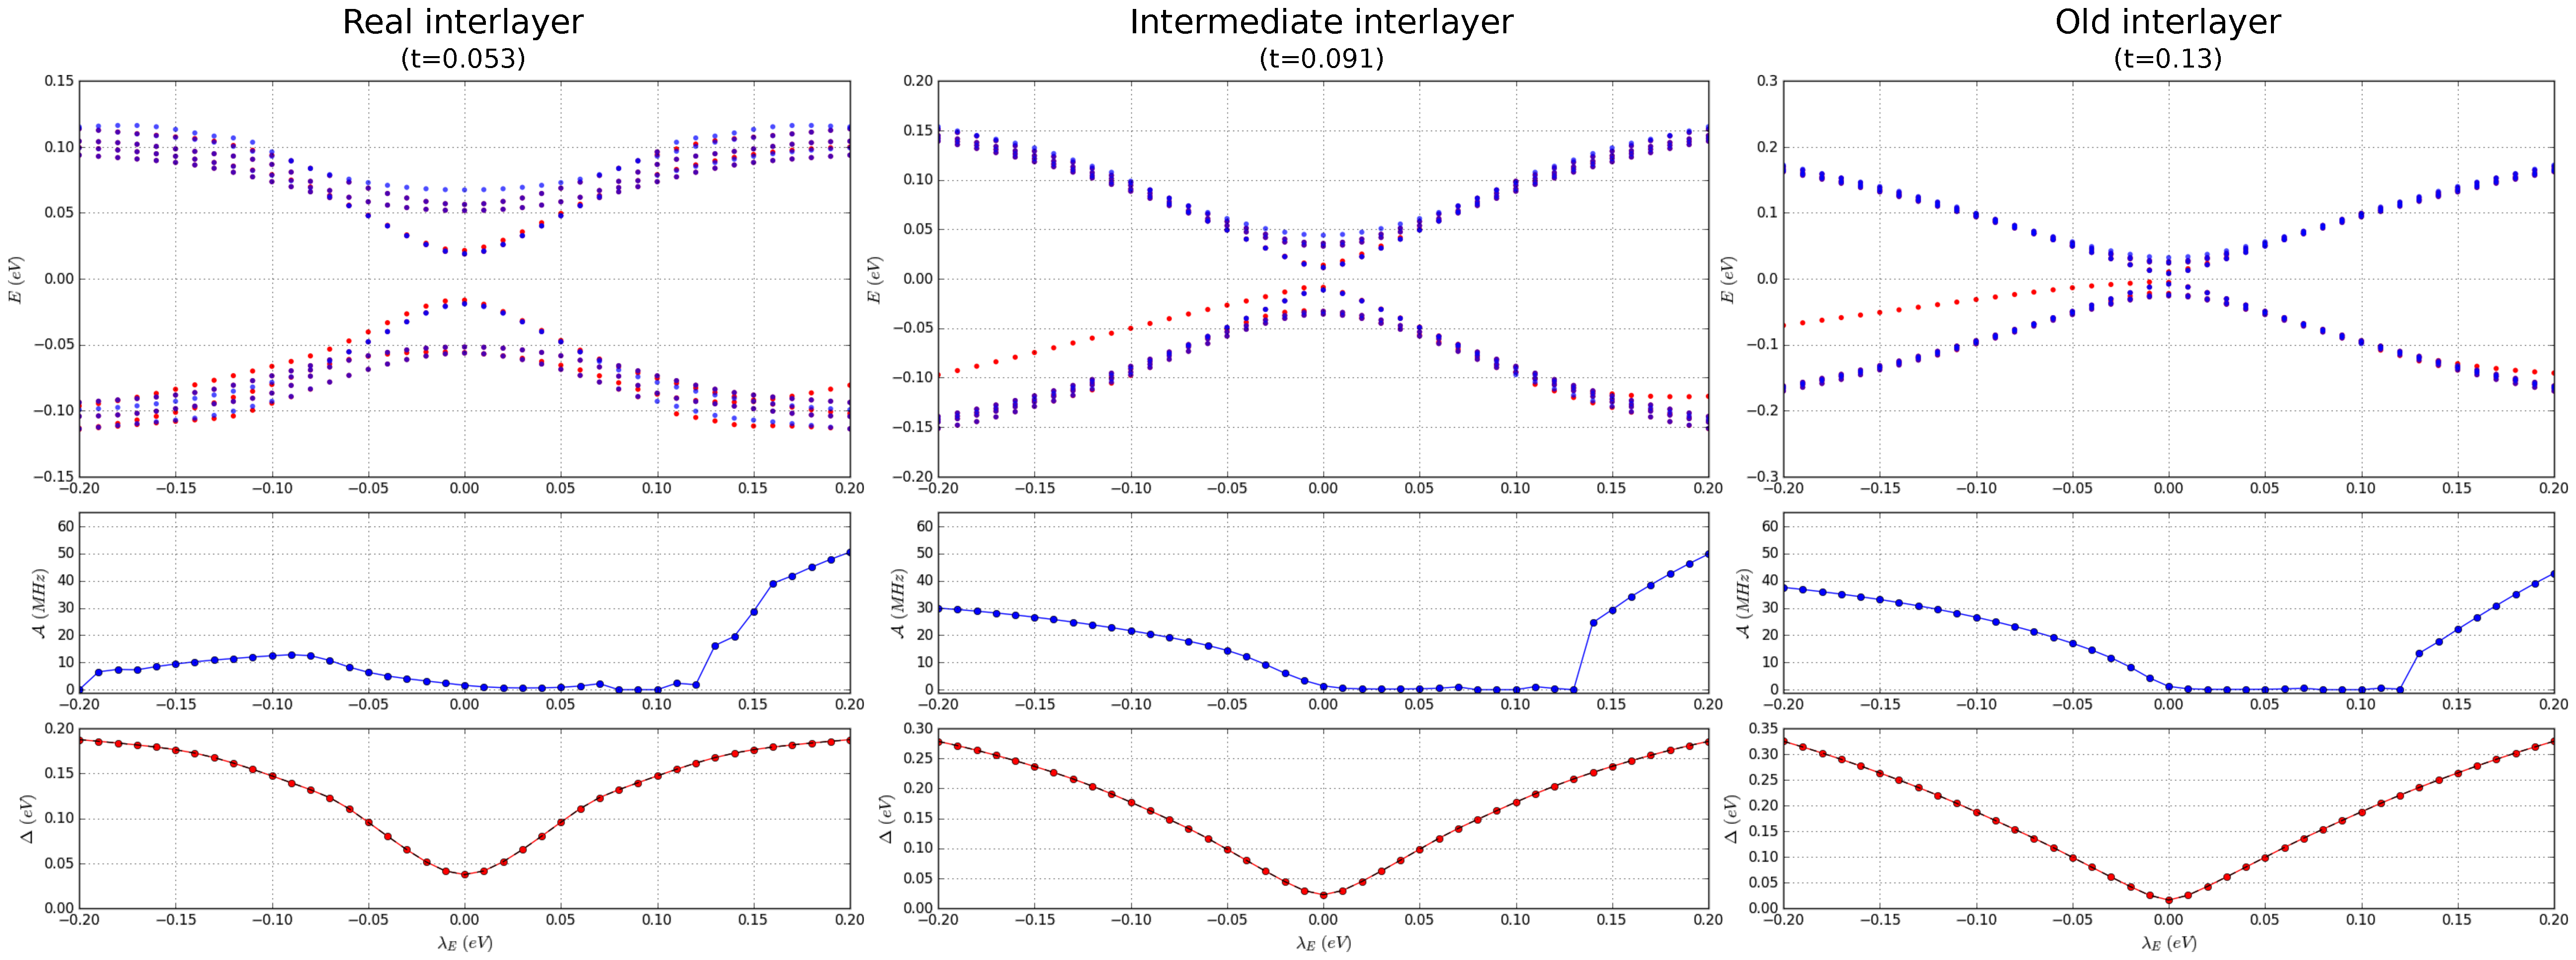
\includegraphics[width=\textwidth]{defects/fig/interlayer_elec.pdf}
%   \vspace{-5pt}
% \caption{Evolution of the low energy spectrum (the 8 eigenvalues closest to $E=0$), the hyperfine coupling and the gap with the electric field for different interlayer couplings. In the first panels the blue dots are the spectrum for the pristine island, without $H$ adatom and the red one is the defected case.}
% \label{spectrums}
% \end{figure}
% \FloatBarrier
% %~~~~~~~~~~~~~~~~~~~~~~~~~~~~~~~~~~~~~~~~~~~~~~~~~~~~~~~~~~~%
% 
% Given an island of a certain size (within the shadowed region in Fig.~\ref{confinement}) the evolution of the spectrum is shown in Fig.~\ref{spectrums}, Notice that the figure \emph{does not show bands} but rather discrete spectrums at different electric fields, in particular, the point at $\Delta_E=0$ \emph{is not the Dirac point}, it is simply the spectrum at zero electric field.
% 
% The main information that we can extract by now from Fig.~\ref{spectrums} is that the electronic structure of graphene bilayer opens a gap with the electric field.
% 
% The real value of the interlayer should be the one in the left panel, and it will be the one used from now on, meaning that \emph{the interlayer coupling will not be a free parameter in our calculations}.
% 
% 
% \section{H adatom on graphene bilayer}
% 
% The physics of a $H$ adatom on bilayer graphene does not differ much from the monolayer case. In this case, again the Lieb's theorem nearly applies, although not exactly since the presence of $s$ orbitals break the bipartite character of the system.
% 
% To strictly recover the vacancy limit we would need to freeze the $s-s$ hopping ($V_{ss\sigma}\to0$) and increase the $s-p_z$ ($V_{sp\sigma}\to\infty$) as well as the on-site of the H atom ($\varepsilon_{H_s}\to-\infty$).
% 
% The effect of having finite hoppings and on-site energy is that the ``zero energy'' state is no longer at $E=0$.
% 
% %~~~~~~~~~~~~~~~~~~~~~~~~~~ FIGURE ~~~~~~~~~~~~~~~~~~~~~~~~~%
% \begin{figure}[h!]
%   \centering
%   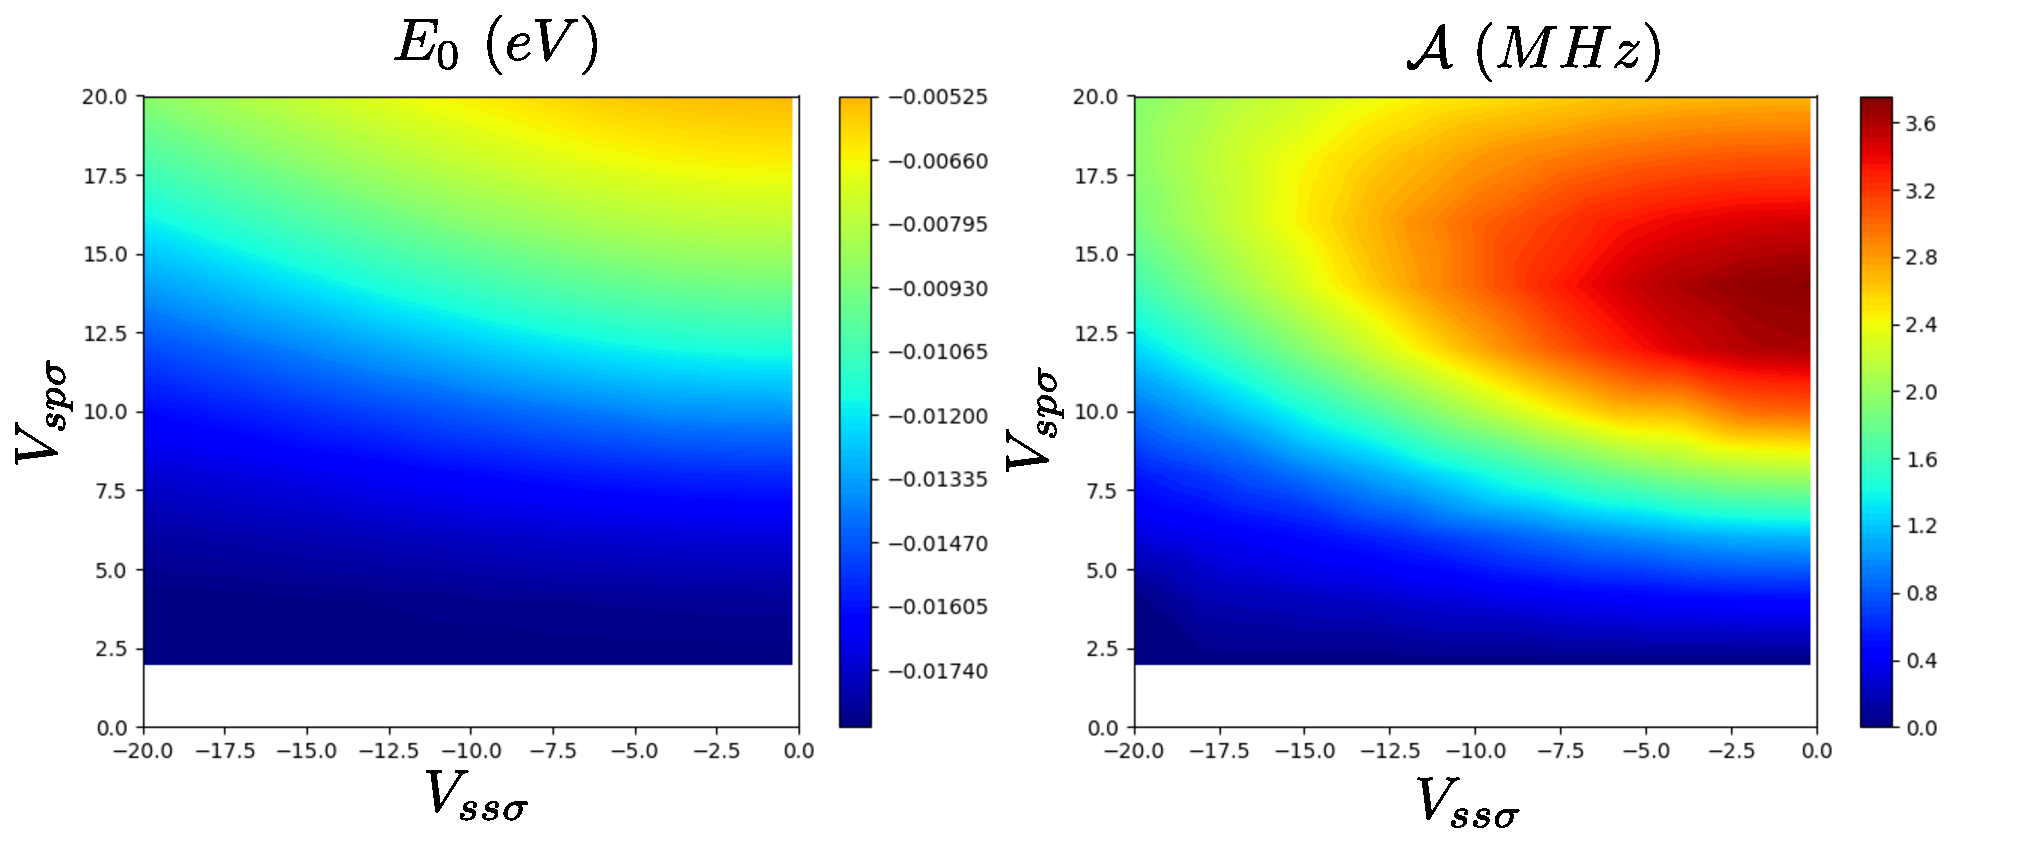
\includegraphics[width=0.9\textwidth]{defects/fig/parameter_space_bi.pdf}
%   \vspace{-5pt}
% \caption{Parameter space for the energy of the in-gap state and the hyperfine coupling for a graphene bilayer nanoisland.}
% \label{SK2d_bi}
% \end{figure}
% \FloatBarrier
% %~~~~~~~~~~~~~~~~~~~~~~~~~~~~~~~~~~~~~~~~~~~~~~~~~~~~~~~~~~~%
% 
% Notice that the parameter space $V_{ss\sigma}-V_{sp\sigma}$ looks quite similar to the monolayer case (Fig.~\ref{SK2d}) although there is a strong reduction in the hyperfine coupling $\mathcal{A}$ since the in-gap state is extended now among roughly twice as many atoms.\\
% 
% 
% Choosing a value of  $V_{ss\sigma}$, $V_{sp\sigma}$ in the higest region in Fig.~\ref{SK2d_bi} we can see the evolution with the electric field:
% %~~~~~~~~~~~~~~~~~~~~~~~~~~ FIGURE ~~~~~~~~~~~~~~~~~~~~~~~~~%
% \begin{figure}[h!]
%   \centering
%   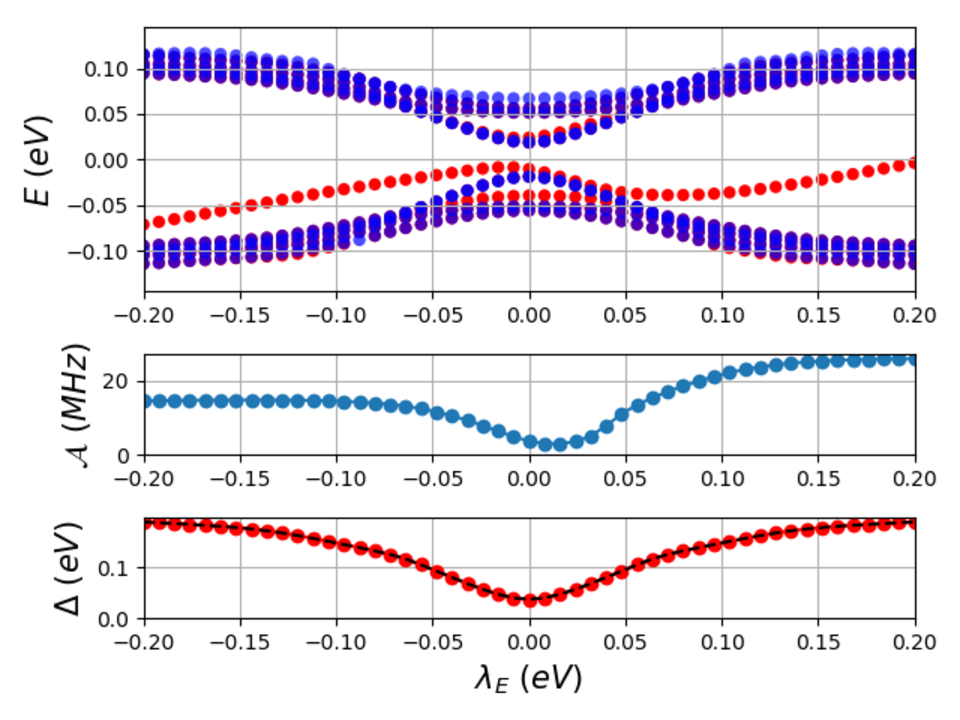
\includegraphics[width=0.6\textwidth]{defects/fig/best.pdf}
%   \vspace{-5pt}
% \caption{Evolution of the 8 eigenstates closest to $E=0$, the hyperfine coupling and the gap with the electric field}
% \label{best}
% \end{figure}
% \FloatBarrier
% %~~~~~~~~~~~~~~~~~~~~~~~~~~~~~~~~~~~~~~~~~~~~~~~~~~~~~~~~~~~%
% 
% 
% And this is what the hyperfine coupling looks like in the parameter space $V_{ss\sigma}-V_{sp\sigma}$ when the electric field is switched on:
% %~~~~~~~~~~~~~~~~~~~~~~~~~~ FIGURE ~~~~~~~~~~~~~~~~~~~~~~~~~%
% \begin{figure}[h!]
%   \centering
%   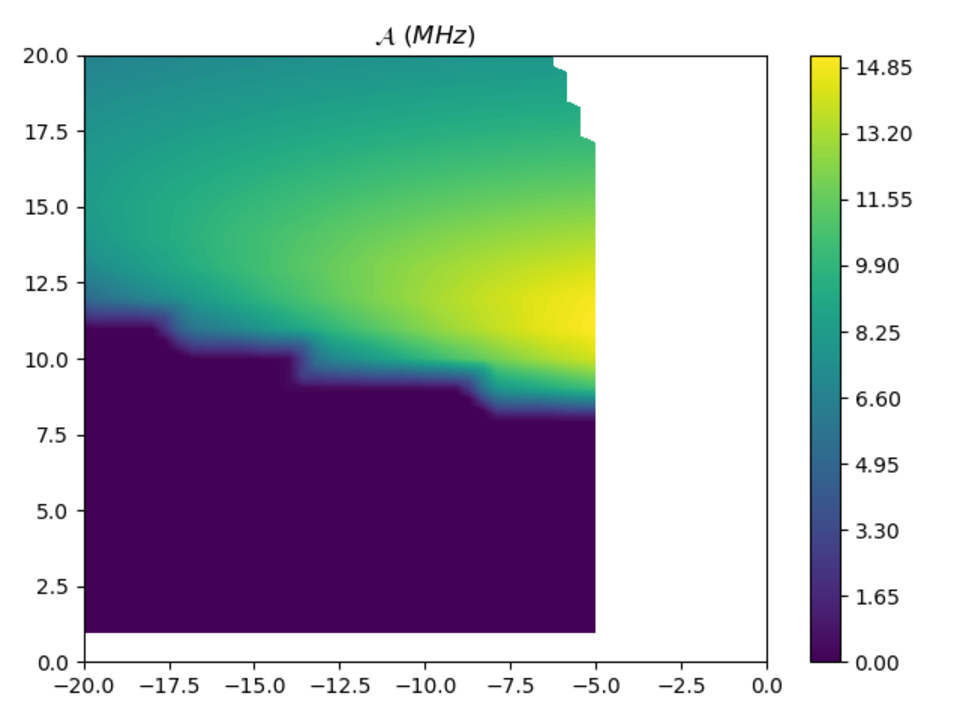
\includegraphics{defects/fig/SK_A_bi_e-02.pdf}
%   \vspace{-5pt}
% \caption{Parameter space for the hyperfine coupling for a graphene bilayer nanoisland in the presence of a strong electric field $\Delta_E=-0.2eV$}
% \end{figure}
% \FloatBarrier
% %~~~~~~~~~~~~~~~~~~~~~~~~~~~~~~~~~~~~~~~~~~~~~~~~~~~~~~~~~~~%
